\documentclass{report}

\usepackage[ruled,vlined]{algorithm2e}
\usepackage{amsmath}
\usepackage{amssymb}
\usepackage{amsthm}
\usepackage{apacite}
\usepackage[toc,page]{appendix}
\usepackage{bbding}
\usepackage{courier}
\usepackage{epigraph}
\usepackage{graphicx}
\usepackage{helvet}
\usepackage[utf8]{inputenc}
\usepackage[switch]{lineno}
\usepackage[normal]{threeparttable}
\usepackage{titlesec}
\usepackage{url}

\newcommand{\beq}{\begin{eqnarray}}
\newcommand{\eeq}{\end{eqnarray}}
\newcommand{\+}{\phantom{-}}

\renewcommand{\labelenumii}{\theenumii}
\renewcommand{\theenumii}{\theenumi.\arabic{enumii}.}

\newtheorem{definition}{Definition}
\newtheorem{property}{Property}
\newtheorem{claim}{Claim}

\DeclareMathOperator{\unif}{unif}
\DeclareMathOperator{\sample}{sample}
\DeclareMathOperator{\setcount}{count}
\DeclareMathOperator{\mode}{mode}
\DeclareMathOperator*{\argmax}{arg\,max}
\DeclareMathOperator*{\argmin}{arg\,min}


%\linenumbers

\author{Edward L. Platt}
\title{Network Deliberation: The role of network structure in large-scale, internet-enabled, participatory decision-making}

\begin{document}

\begin{titlepage}
   \begin{center}
       \vspace*{1cm}

       \textbf{\Large Network Deliberation: The role of network structure in large-scale, internet-enabled, participatory decision-making}        
            
       \vspace{1.5cm}

       \textbf{Edward L. Platt}
       
       \today

       \vfill
            
       Dissertation Proposal\\
       Doctor of Philosophy \\
       University of Michigan \\
       School of Information
            
       \vspace{0.8cm}
     
            
   \end{center}
    {\bfseries Doctoral Committee:}\\
    Associate Professor Daniel M. Romero \\
    Professor Scott E. Page \\
    Associate Professor Tawanna Dillahunt \\
    Assistant Professor Ceren Budak
         
\end{titlepage}

%\begin{abstract}
%% This is the template for submission of abstracts to NetSci 2017 in Indianapolis, IN.
% It is modified from NetSci 2016.
% The editor of the booklet reserves the right to modify your submission.

%% To process this file run LaTeX2e

%%********DO NOT EDIT****************
\documentclass[12pt]{article}
\usepackage{mathptmx}
\usepackage{graphicx}
\pagestyle{empty}

\setlength\topmargin{0pt}
\addtolength\topmargin{-\headheight}
\addtolength\topmargin{-\headsep}
\setlength\oddsidemargin{0pt}
\setlength\textwidth{\paperwidth}
\addtolength\textwidth{-2in}
\setlength\textheight{\paperheight}
\addtolength\textheight{-2in}
\usepackage{layout}

\renewcommand{\title}[1]{\noindent\textbf{#1}\bigskip\\}
\renewcommand{\author}[1]{\noindent #1\bigskip\\}
%%***********************************

\begin{document}

%**********USER DEFINED**************
%Enter title here
\title{Towards Attack-Tolerant Networks: Multipath Fault Tolerance}
%Enter author(s) and address here
\author{Edward L. Platt$^1$ and Daniel M. Romero$^1$\bigskip\\
{\small
1. University of Michigan, Ann Arbor, MI, USA\\
}
}
%Enter abstract here
Centralized systems are susceptible to
targeted attacks against central points,
suggesting the importance of decentralization in attack-tolerant systems.
While many techniques exist for tolerating random faults,
better techniques for tolerating {\em adversarial faults} such as targeted attacks are needed.
In communication networks, targeted attack can leave users vulnerable to
censorship and surveillance of messages at central points.
Even when encryption is used, it can be bypassed by coercion, e.g., subpoenas.
While decentralized {\em protocols} have become a popular approach to attack-tolerance, centralized network {\em
structure} can arise even when protocols are
decentralized.
Despite their decentralized protocols,
the internet and World-Wide Web have
been shown both theoretically and historically to be highly susceptible to
adversarial faults [1], in part due to emergent structural centralization.
In this work, we present
1. A fault tolerace scheme for networked communication having a failure probability that decreses exponentially with the number of available independent paths;
2. A routing algorithm for constructing such indpendent paths in the butterfly network topology [2]; and
3. A bounded-transitivity trust model that makes it possible to quantify the adversarial fault tolerance of a network.
Our work is the first theoretical demonstration of a point-to-point communication network architecture able to tolerate coercion and other
targeted attacks, without requiring infinitely transitive trust.
We also evaluate the fault tolerance of an imperfectly implemented butterfly topology by partially rewiring a snapshot of the internet's router network.
We find that rewiring only 10\% of the edges allows the network to withstand faults in the most central 2\% of nodes,
increasing to 8\% of nodes for 90\% rewiring.
Our results show that it is possible, in principle, to create highly attack-tolerant communication systems that can withstand targeted and coercive attacks, but only when it is possible to influence network structure.
\begin{figure}[!h]
\begin{center}
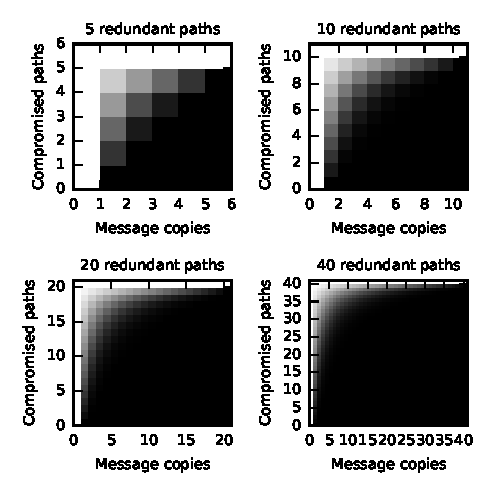
\includegraphics[scale=0.75]{fig-perror}
\end{center}
\caption{
Failure probability decreases rapidly with the number of
message copies, and increases slowly with the number of faults.
Messages are difficult to attack and easy to defend.
}
\end{figure}

\noindent[1] R. Albert et al. Error and attack tolerance of complex networks. {\em Nature,} 406(6794), 2000.
\\
\noindent[2] A. D. Kshemkalyani and M. Singhal. {\em Distributed Computing}. Cambridge U. Press, 2008.


% Place the abstract of your talk/poster here, 250 Words maximum.
% Mathematical formulae may be set in LaTeX, but do NOT use the
% bibliography environment -- if you must have references, use an 
% enumerated list.
%
% Your abstract (plus one figure) should not exceed one page.
%
% Check carefully.

%************************************
\end{document}
%\end{abstract}

\tableofcontents

\listoffigures
\listoftables

\chapter{Introduction}
\label{chap:intro}
The ability of large groups to reach mutually agreeable decisions is key to
democratic governance, social movements, and peer production (e.g., Wikipedia).
Faced with the intractability of large-scale decision-making, traditional
systems have sacrificed one or more desirable properties, such as participation
(as in representative democracy), deliberation (as in voting), equality
(as in command hierarchies), and speed (as in formal consensus).
This dissertation examines the emerging role of internet-enabled collaborative
networks in overcoming these historical limitations.

In recent years, examples of large-scale collaborations have emerged that seem
to achieve the previously unachievable. Millions of volunteer Wikipedia editors
have created a high-quality encyclopedia without centralized leadership
\cite{keegan_evolution_2017, giles_internet_2005}.
The Free Software movement has produced the Linux kernel and GNU operating
system, which power much of the modern internet
\cite{coleman_coding_2013, benkler_coases_2002, raymond_cathedral_1999}.
Social movements such as the Arab Spring, Occupy, Black Lives Matter, and
Podemos have reshaped national governments and brought attention to deeply
entrenched social issues
\cite{tufekci_twitter_2017, gonzalez-bailon_networked_2016}.
The emergence of these large-scale decentralized collaborations has been
attributed to the fast, bidirectional,
and global communication enabled by the internet
\cite{tufekci_twitter_2017, benkler_coases_2002}.
A better understanding of how specifically such communication sidesteps
historical barriers to large-scale collaboration will contribute to more
effective policy as well as best practices for organizational design and
intervention.
This dissertation focuses on one particularly challenging aspect of
such collaborations: decision-making
I specificaly examine how,
when groups are too large for all members to participate in all discussions,
the course and outcome of the decision-making process is influenced by the
communication network structure: the shape of who talks to whom.

\section{Theoretical Framework}

This dissertation draws on ideas from network science, economics, and complex
systems.
While a topic as broad as decision-making can be studied from many perspectives,
these fields provide a minimal framework for studying how individual preferences
and behaviors interact with interpersonal communication networks to influence
group decisions.

The fundamental challenge of large-scale collective decision-making is how to
reconcile the conflicting preferences of individual group members.
This challenge has been studied formally in social choice theory,
a sub-field of economics.
Prior work in social choice theory has found, somewhat discouragingly,
that even when all individual preferences are known perfectly,
making a fair collective decision isn't always possible.
In some cases, the method of aggregating individual preferences
(i.e. the voting system) can influence the outcome.
Social choice theory focuses on understanding of these limitations,
such as the Condorcet Paradox
\cite{condorcet_essay_1785} and
Arrow's Impossibility Theorem \cite{arrow_social_2012}.
This dissertation finds hope in the transformative potential of the
deliberative process.
Social choice theory typically assumes fixed individual preferences.
Deliberation allows individuals to influence and change each other's
preferences,
which creates the potential to sidestep the historical limitations of
social choice theory.
When individual preferences are allowed to vary, it becomes possible for an
irreconcilable set of preferences to evolve into one with a clear winner.
So far, this possibility has received relatively little attention,
most likely due to the historical intractability of large-scale deliberative
decision-making.
This dissertation explores the potential of the internet to enable effective
deliberation in large collectives.
Such large-scale deliberation creates the potential for members to
resolve conflicting preferences and reach mutually acceptable decisions
without relying on coercive or hierarchical processes that might introduce
power imbalances or informational biases.

Network science provides the tools for analyzing the structure of interpersonal
networks.
Interpersonal interactions in large collaborations are necessarily structured:
when a group is too large for each individual to interact with all other individuals,
the question of ``who talks to whom?'' creates a network structure.
By modelling collaborative groups as a collection of abstract ``nodes''
connected by interpersonal communication links,
a group's communication structure can be studied in isolation.
Findings from network science suggest that social processes on networks can be
influenced by structural properties such as
the {\em degree}: the number of links a node has,
{\em geodesic distance} the number of links separating two nodes,
and {\em clustering}: how common it is for two linked nodes to share links with
a third \cite{boccaletti_complex_2006}.
While network structure is certainly not the only factor to influence collective
decision-making,
studying network structure in isolation provides a baseline for the
further study of social dynamics and other non-structural factors.
Network structure is also significant as a potential point of intervention in
cases where social dynamics may be difficult to influence.

This dissertation also incorporates theoretical and computational models from
social learning theory.
Social learning theory acknowledges that individuals rarely
learn or make decisions in isolation, but rather learn from and imitate others
in their social network
\cite{golub_naive_2010}.
Social learning theory
formalizes both the types of tasks collectives perform
\cite{hong_interpreted_2009}
and the behavioral strategies individuals might employ
\cite{lazer_network_2007, barkoczi_social_2016}.
These strategies range from pure imitation to critical evaluation,
depending on the circumstances being modeled.
Social learning models provide a baseline to compare empirical observations
against,
as well as a language and framework for contextualizing findings.

Throughout this dissertation,
I motivate and develop a novel theoretical framework,
which I call {\em network deliberation}.
My review of the literature identifies a common theme
among successful large-scale internet-enabled collaborations:
large collectives composed of interlocking smaller groups.
These groups have various names, including:
committees, working groups, teams, circles, cores, syndicates,
affinity groups, zones, and nodes.
As an abstraction of these small interlocking group, I will use the term "pods."
Network deliberation describes large-scale collective deliberation achieved
through interlocking pods.
As in the theories of interlocking directorates \cite{levine_study_1979},
interlocking publics \cite{habermas_structural_1991},
and network rotation \cite{salehi_hive_2018},
pods allow for beneficial small group dynamics,
while the overlap between pods enables diffusion of information and opinions
through the greater collective.
In network deliberation, the method of assigning individuals to pods
(whether deliberate or self-organized) can produce interpersonal networks with
varying structures.
The central question of this dissertation is how the structure of these
interlocking-pod networks influences the process and outcome of deliberation
in large collaborations.

\section{Methodology}

Studying collective behavior on the scale of hundreds, thousands, and millions
presents significant methodological challenges.
To address these challenges, this dissertation combines multiple methodologies,
including: observational study, agent-based modelling, and field experiment.
I use observational studies to reconstruct real-world collaborative networks
from the English-language Wikipedia and analyze the collaborative output of
those networks (Chapter \ref{chap:wp-prod-perf}).
Observational study has the benefits of scaling to millions of individuals
in a real-world environment.
However, observational studies typically cannot establish causal relationships,
only correlation.

To begin to address the causal relationship between network structure and
deliberative outcome, I use agent-based models
(Chatpers \ref{chap:wp-prod-perf} and \ref{chap:abm}).
Agent-based models are computational models of large systems composed of
many agents following simple behavioral rules.
In this case, agents represent individual collaborators,
and their behavior is determined by their preferences and their strategy for
incorporating information learned from their neighbors.
Agent-based models can establish causality,
and do so in group sizes limited only by available computing power.
As simplified models, however, their results cannot necessarily be generalized
to real-world scenarios.

To bridge the limitations of the above methods,
this dissertation will include a controlled field experiment evaluating the
effect of network deliberation in real-world collective decision-making
(Chapter \ref{chap:experiment}).

\section{Contributions}
This dissertation describes the contributions of three projects.
Chapter \ref{chap:wp-prod-perf} describes an observational and computational
study of WikiProjects on the English-language Wikipedia,
and reports the following contributions:
\begin{itemize}
\setlength\itemsep{0pt}
\item Despite an overall productivity/performance trade-off,
WikiProjects with low-degree coeditor networks tend to have both higher
productivity and higher performance;
\item Short geodesic lengths are associated with higher performance,
consistent with a conformity-based learning strategy;
\item Structural inequality, as measured by degree skewness,
is associated with lower performance;
\item The agent-based model shows that the productivity and performance of
collaborations can depend on network degree,
and that the direction of that dependence can depend on social learning strategy.
\end{itemize}

Chapter \ref{chap:abm} describes an agent-based model of network deliberation,
comparing performance across several network topologies and social learning
strategies.
The primary contributions are:
\begin{itemize}
\setlength\itemsep{0pt}
\item When agents conform to social influence,
Network deliberation identifies solutions of higher quality than
conventional deliberation,
while requiring less time to converge.
\item Within network deliberation conditions,
the structurally-efficient random pod network outperforms the
structurally-inefficient long-path network when agents conform to social influence.
However, when agents prefer their own judgement to social influence,
the inefficient network yields higher performance,
consistent with findings for conventional networks.
\cite{barkoczi_social_2016}.
\item A novel social learning strategy, confident-neighbor,
which outperforms or matches the conventional best-neighbor strategy across all
networks considered,
despite using strictly less information about solution quality.
\end{itemize}

Chapter \ref{chap:experiment} proposes and describes current progress on a
field experiment to study network deliberation in large-scale human collaborations.
The study design uses periodic ranked-choice polls to track individual preferences
throughout the course of a large-scale online deliberation.
By varying communication network structure and tracking the evolution of individual
preferences,
this experiment evaluate the ability of network deliberation to resolve conflict
and build consensus, relative to conventional single-group deliberation.

\section{Dissertation Progress and Timeline}
At the time of this proposal,
the analysis of English-language WikiProjects described in Chapter
\ref{chap:wp-prod-perf} has been completed and resulted in a published
paper \cite{platt_network_2018}.
The agent-based modelling project described in Chapter \ref{chap:abm}
has been completed and resulted in a finished manuscript.
I have completed custom software, obtained IRB exemption, and conducted
several pilot studies for the field experiment described in
Chapter \ref{chap:experiment}.
I expect to have data collected from at least one full-scale experiment
by the end of 2021, and to have the data analyzed by mid-February, 2022.
I plan to have my dissertation completed by mid-May, 2022.


\chapter{Network structure, productivity, and performance in WikiProjects}
\label{chap:wp-prod-perf}
\epigraph
{The problem with Wikipedia is that it only works in practice. In theory, it's a total disaster.}
{---Gareth Owen \cite{elsharbaty_editing_2016} }

The internet has enabled collaborations at a global scale.
Wikipedia, a free encyclopedia that invites anyone to edit articles,
is one of the most successful and visible examples of such a collaboration.
Organizing groups without top-down control is notoriously
difficult
\cite{freeman_tyranny_1972},
and yet Wikipedia, with millions of self-organized editors,
has produced a high-quality encyclopedia \cite{giles_internet_2005,keegan_evolution_2017}.
A better theoretical understanding of projects like Wikipedia is highly desirable as it could
help inform the design of new collaborative projects.
We focus on one aspect of a large-scale decentralized collaboration:
its network structure \cite{newman_structure_2003}.
How does Wikipedia's non-hierarchical structure relate to its success?

We look at WikiProjects on the English-language Wikipedia.
WikiProjects are collections of thematically related articles,
each with their own standards and norms.
When measuring the quality of collaborative projects,
there are at least two distinct measures to consider.
The first measure is short-term:
how effective a unit of work is at improving
the collaboration's output,
which we call {\em productivity}.
The other measure is long-term:
the highest quality typically reached by an output,
which we call {\em performance}.
These two terms are often used interchangeably,
but we find it fruitful to distinguish between the two.
We find that Wikipedia exhibits an overall trade-off between performance and productivity.
However, some WikiProjects surpass others in both productivity and performance,
suggesting the existence of factors that correlate positively with both.

Our study focuses on the coeditor networks of each WikiProject:
which editors have edited at least one article in common?
These relationships represent the possible flow of information.
We focus specifically on mean degree, degree skewness, and path length.
High-degree editors have more collaborators,
which can increase diversity and access to information at the possible
expense of higher coordination costs
\cite{hong_groups_2004,golub_naive_2010}.
Highly skewed degree distributions can amplify the biases of high-degree
editors while reducing the need for explicit coordination
\cite{kearns_experiments_2012}.
Networks with shorter path lengths allow information to travel more quickly
at the possible expense of less local diversity
\cite{mason_propagation_2008,barkoczi_social_2016}.

In addition to our empirical study,
we use agent-based modeling to examine the consequences of specific
assumptions on networked collaboration.
We model individual behavior using a {\em social learning strategy} that
assumes agents 1. can only access a fraction of the model's state,
2. interact with others who share their concerns,
and 3. integrate their preferences into a single state.
Our model is the first we are aware of to incorporate these assumptions,
which are present across many real-world collaborations,
including Wikipedia.

Our main findings are:
\begin{itemize}
\setlength\itemsep{0pt}
\item Despite an overall performance/productivity trade-off,
WikiProjects with low-degree coeditor networks tend to have both higher performance and higher productivity;
\item Short paths are associated with higher performance, consistent with a conformity-based learning strategy;
\item Structural inequality, as measured by degree skewness, is associated with lower performance;
\item Our agent-based model
shows that the productivity and performance of collaborations can
depend on network degree,
and that the direction of that dependence varies with social learning strategy.
\end{itemize}

Our findings shed light on the importance of network structure for successful
collaboration.
These findings might be informative for future interventions that
recommend tasks based on how they will
influence network structure,
or for interventions that seek to encourage behaviors
complementary to existing network structure.

\section{Background and Related Work}
\label{sec:background}
The present paper investigates the relationship between social networks
and collaboration outcomes.
This connection has been explored by a number of theoretical,
numerical, and small-scale lab studies in the field of
{\em social learning}.
We contribute to this literature with a large-scale, empirical field study.
In much of the existing literature,
degree distribution correlates with outcome measures.
But aside from the naive Bayes case, it is unknown whether
the correlation is explained best by degree or by another structural property, such as characteristic path length.
In the empirical networks we study,
unlike artificial networks,
the structural properties vary independently,
making it easier to isolate individual
network properties that correlate with outcome variables.

{\bf Social Learning.} In {\em networked social learning},
agents are represented by nodes on a network
and can interact only with their neighbors.
Social learning tasks can be divided into cases where agents have {\em generated signals}
(independently noisy estimates of a true value)
and those where agents have {\em interpreted signals}
(solutions based on different selections of available data)
\cite{hong_interpreted_2009}.
The behavior of individual agents is described by their
{\em social learning strategy}.
For generated signals,
a naive Bayesian approach converges to the truth
when all agents have the same degree,
while the speed of convergence depends on the {\em spectral gap}
between the two largest eigenvalues of the network's interaction matrix
\cite{degroot_reaching_1974,golub_naive_2010}.
Complex social learning tasks can also be modeled as the problem
of maximizing an objective function with many local maxima,
referred to as a {\em rugged landscape}
\cite{lazer_network_2007,mason_propagation_2008,mason_collaborative_2012,grim_scientific_2013,barkoczi_social_2016}.
Numerical simulations have shown that efficient networks
(those with short paths between nodes)
can result in faster convergence at the cost of a less optimal solution,
due to less time for exploration
\cite{mason_propagation_2008,grim_scientific_2013}.
However, when conformity-based social learning strategies are used,
efficient networks can sometimes find more optimal solutions than
inefficient ones \cite{barkoczi_social_2016}.
Using an agent-based model, Hong and Page \cite{hong_groups_2004} found that
diverse groups can outperform groups composed of the best individual
problem-solvers.

{\bf Lab experiments.} Lab-based experiments on networked collaboration
suggest a complex interaction between network topology and other factors.
While groups of networked human subjects perform very well on
difficult graph-coloring tasks, the best performing network architectures
(e.g., fully-connected vs. small-world) vary
from task to task \cite{kearns_experiments_2012}.
The same studies found that while human subjects tend to perform well on
many networks, they perform worst on self-organized
networks, possibly due to higher structural inequality
(degree skewness).
Similarly, some network topologies are able to reach faster decisions in the
presence of more information, while others show the opposite effect
\cite{kearns_experimental_2006}.
Based on lab experiments, Fowler and Christakis \cite{fowler_cooperative_2010}
suggest that individual decisions towards altruism are conditional on their
neighbor's behavior and ``contagious'' up to three degrees away.
Later experiments by Suri and Watts \cite{suri_cooperation_2011} confirmed the
existence of conditional altruism,
but concluded that altruism
influences only first-degree neighbors.

{\bf Digital Communities.}
Research on digital communities has also examined the role of 
diversity and inequality
in collaborative work and decision-making.
In sociology, research has focused on the relationship between
network structure and social capital.
Powerful individuals are often ``brokers''
who act as exclusive intermediaries between disconnected portions of the
social network \cite{silverman_patronage_1965}.
Similarly, successful innovation in organizations often occurs in ``structural
holes'' between groups \cite{granovetter_strength_1973}.

For Wikipedia specifically,
Robert and Romero \cite{robert_crowd_2015} found that
larger group sizes yield higher article ratings
when the groups are diverse and experienced. Kittur and Kraut found that different types of coordination have a complex
effect on the quality of Wikipedia articles \cite{kittur_harnessing_2008}.
Both explicit and implicit coordination result in higher quality articles,
with explicit coordination being especially central in the early life of an
article.
Shaw and Hill \cite{shaw_laboratories_2014}
found that behavior in online wiki communities is consistent
with the ``iron law of oligarchy,''
which states that
earlier members of a group will, over time, gain disproportionate
decision-making power and act increasingly out of self-interest rather than
the good of the group \cite{michels_political_1999}.
Similarly, Halfaker et al. \cite{halfaker_rise_2013} attributed decreasing
participation on Wikipedia to poor retention of new users.
Looking specifically at Wikipedia policies determined by editor consensus,
Keegan and Fiesler \cite{keegan_evolution_2017} found a trend
from flexible rule-making towards less flexible maintenance and deliberation.
Using content analysis,
Morgan et al. \cite{morgan_project_2013} found WikiProjects to be
more loosely organized than traditional teams.

Across the broad range of work discussed above,
a few key themes emerge.
Both the productivity and the performance of a collaboration are important
considerations and vary depending on both network structure and type of task
\cite{kearns_experiments_2012}.
While generated signal models of social learning predict no relationship
between the two
\cite{golub_naive_2010},
contagion-style innovation models predict a trade-off
\cite{mason_collaborative_2012,barkoczi_social_2016}.
Such a trade-off has been observed in simulations and lab experiments on
collaboration
\cite{kearns_experiments_2012,grim_scientific_2013}.

\section{WikiProjects}
\label{sec:wp}

Many articles on Wikipedia belong to one or more WikiProjects.
WikiProjects are groups of thematically-related articles
(e.g., articles related to Philosophy).
Information about an article's associated WikiProjects
can be viewed on that
article's talk page (Figure \ref{fig:knitting}).
Each WikiProject has its own page and talk page,
containing information about conventions within the project
as well as discussions about individual articles.
WikiProjects are thus distinct communities, with distinct norms and processes.
These communities are the fundamental units of analysis in this paper.

One of the main roles of a WikiProject is to evaluate the quality of its articles.
Quality assessments are made through consensus-based deliberation on the WikiProject
talk page.
Within a WikiProject,
assessments are typically made using the following {\em assessment classes}
(in order of increasing quality):
Stub, Start, C, B, A.
Different WikiProjects can assign different quality assessments to the same
article.
Differences between quality assessments could reflect different quality standards,
different grading systems, different responsiveness to changes in an article, etc.

In addition to the above assessment classes, articles on Wikipedia can be tagged as
``good article'' (GA) or ``featured article'' (FA) quality.
FA and GA determinations are made using a Wikipedia-wide consensus,
independently of WikiProject-based evaluations.
FA articles are ``the best articles Wikipedia has to offer''
\cite{wikipedia_contributors_wikipedia:featured_2018}.
GA articles meet ``a core set of editorial standards`` but are ``not featured article quality''
\cite{wikipedia_contributors_wikipedia:good_2017}.
When an article is assigned GA or FA status,
WikiProject quality assessments are often updated to reflect that status.
For example, the article {\em Mewtwo} was assessed as GA status on October 5,
2009 and shortly afterwards
its quality assessment was changed from B to GA within both
{\em WikiProject Pok\'emon} and
{\em WikiProject Video Games}.
This example also illustrates a quirk of conventions on Wikipedia:
very often, articles pass to GA or FA directly from B, skipping A.
The majority of WikiProjects rarely use the A class quality assessment.

\begin{figure}[t!]
\begin{center}
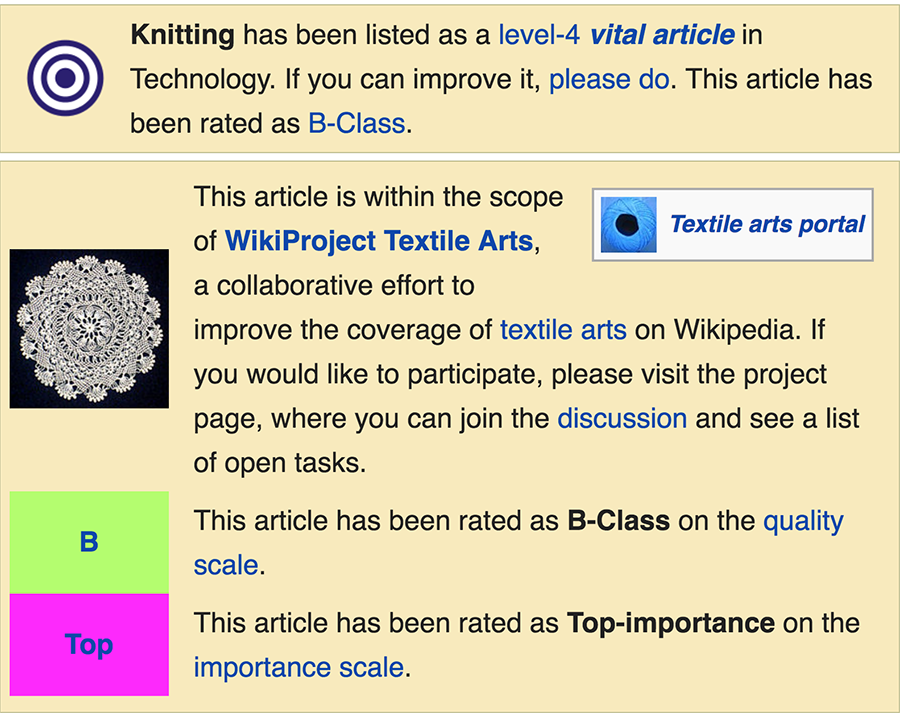
\includegraphics[width=3in]{fig/WPProdPerf/fig-knitting.png}
\caption{
From Wikipedia {\em Knitting} talk page.
Two WikiProjects have assessed the article as B-class quality.
\label{fig:knitting}
}
\end{center}
\end{figure}

\subsection{Data}

Our analysis combines multiple data
sets from the English-language Wikipedia \cite{platt_english_2018}.
For information about edit history, we used a publicly-available data set containing
metadata (time, article id, user) about all edits from July 12, 2006 to December 2, 2015.
We used a custom script to scrape article quality assessments from logs produced
by WP 1.0 Bot for 2279 unique WikiProjects
between May 4, 2006 and December 2, 2015.
Finally, we used a publicly-available database dump of page events (including rename events)
to reconstruct the article id for each title mentioned in the assessment logs.

\subsection{Productivity and Performance}

When individuals collaborate to solve a problem,
there are many ways to gauge their success.
One possibility is {\em productivity}:
how quickly they find a solution.
Another is {\em performance}:
how good their solution is.
Evidence from numerical simulations
\cite{lazer_network_2007,mason_propagation_2008,mason_collaborative_2012,grim_scientific_2013,barkoczi_social_2016},
lab studies \cite{kearns_experiments_2012},
and field observations \cite{gentry_consensus_1982}
all suggest a trade-off between productivity and performance.
While common, this trade-off is not absolute,
suggesting it is sometimes possible to simultaneously increase
performance and productivity.
The identification of factors associated with both higher productivity
and higher performance has obvious practical importance.
In this paper, we focus on how network structure
relates to productivity and performance within WikiProjects.

For a WikiProject, productivity quantifies how much participants can raise the
assessed quality of an article for a fixed amount of work.
We measure work by the number of revisions made.
Quality assessments are made through consensus of the project participants themselves.
Different projects can have different standards and practices for assessing article quality,
so the productivity is not a measure of how quickly some objective measure of quality improves,
but rather of how quickly the project participants can reach consensus on the improvements that
need to be made and make those improvements.
Because our definition relies on assessment transitions,
we must define productivity variables for
each of the project-level quality assessments: A, B, and C.
For a particular grade $G$,
we desire our definition of productivity to meet the following conditions:
\begin{itemize}
\setlength\itemsep{0pt}
\item{Strictly increasing in the number of articles reaching grade $G$ (with revision count fixed);}
\item{Strictly decreasing in the number of revisions (with transition count fixed);}
\item{Independent of WikiProject size: not affected by adding an article having the same productivity.}
\end{itemize}

We now define an productivity measure which meets the above criteria.
Let $T(W,G)$ be the set of article assessment transitions from below grade $G$
to grade $G$ or higher in project $W$.
Let $N(W,G)$ be the number of articles in project $W$ which ever transition
from below grade $G$ to grade $G$ (or higher).
Given a transition $t$,
let $r(t)$ be the number of revisions to the article
since its previous grade transition,
and let $g(t)$ be the number of grade levels crossed bt $t$.
We quantify the productivity $E(W,G)$ as the inverse of the mean number of revisions
per transition:
\beq
E(W,G)
&=&
\left[
\frac{1}{
N(W,G)
}
\sum_{t \in T(W,G)} \frac{r(t)}{g(t)}
\right]^{-1},
\eeq
where the $g(t)$ term accounts for assessments that raise article quality by
several grades by
dividing the revisions evenly between all grade levels achieved.

For performance, we wish to quantify how good articles tend to be when they reach a stable state.
Measuring performance is difficult for two reasons:
there is no objective measure of article quality available,
and articles are always changing, making it difficult to know which articles should be considered
complete or stable.
We use an extremely simple performance measure that gives surprisingly consistent results.
In addition to per-project quality assessment, articles can be given ``featured article'' or
``good article'' status.
The criteria for these statuses are consistent across all of Wikipedia,
and any editor can participate in the discussion and decision to award good or featured
status.
In other words, the good and featured statuses are less subjective than per-project assessments.

Our performance measure $P(W)$ is defined simply as
the percentage of articles in project $W$ which have reached
good or featured status:
\beq
P(W) &=& \frac{f(W) + g(W)}{n(W)},
\eeq
where $f(W)$ and $g(W)$ are the numbered of featured and good articles respectively,
and $n(W)$ is the total number of articles.

\subsection{Coeditor Networks}

We would like to determine how the social network structure of
Wikipedia---the pattern of who interacts with whom---relates to
productivity and performance.
There are several types of interactions we could focus on,
including:
coediting, user talk messages, and talk page replies.
We choose to focus on coediting: when two editors have made changes to the
same article or talk page.
While editors can communicate directly through user talk messages,
the number of such messages is small compared to the number of edits to article
and talk pages.
We also could have considered direct replies between editors on article talk
pages, but these replies are typically seen (and intended to be seen)
by everyone reading the talk page,
and are part of larger conversations.
When an editor views a page,
they are potentially viewing content from and interactions
between all editors who came before them,
motivating our choice to focus on the social network structure of
coeditors.

The {\em coeditor network} of a WikiProject consists of nodes representing editors
and edges connecting pairs of editors who have edited the same article.
The edges are directed, with the direction representing
{\em plausible information flow};
an edge from Alice to Bob exists if Alice edited an article and then Bob edited the same article at
a later time. Note that edges can exist in both directions. 
We make the simplifying assumption of unit weight for all edges.
We focus on three structural properties:
degree, characteristic path length, and min-cut.
Degree and characteristic path length have been shown to correlate with
performance and productivity in some social learning settings
\cite{golub_naive_2010,mason_propagation_2008,grim_scientific_2013},
while min-cut can be interpreted as a measure of decentralization,
common feature of peer-produced communities such as Wikipedia
\cite{benkler_wealth_2006}.

The degree distribution is the simplest network property we analyze.
The in-degree (out-degree) of a node is the number of edges to (from) that node.
Taking the average of either in-degree or out-degree gives the same value:
the {\em mean degree} of the network.
In our context, the mean degree represents, on average,
how many other editors each editor has collaborated with.
We also consider the {\em skewness} of the in-degree and out-degree distributions.
A large positive degree skewness for a WikiProject coeditor network
implies that a small number of editors have a very large number of collaborators,
while a small positive value implies that the editors having the most collaborators
don't have many more than a typical editor.

We also calculate the characteristic path length for each WikiProject coeditor network.
The {\em distance} from node $s$ to node $t$ is the distance of the shortest path
from $s$ to $t$.
The {\em characteristic path length} (or just {\em path length})
is the mean distance between all editor pairs,
excluding unconnected pairs.
To account for unconnected nodes, we also measure the {\em connected fraction}:
the fraction of ordered node pairs with a directed path from source to sink.
The path length represents how quickly information can move through the network.
Networks with longer paths require more interactions for information to propagate,
which has been shown to reduce productivity in some settings
\cite{mason_propagation_2008,barkoczi_social_2016}.

Our final network measure quantifies the connectivity of a project's coeditor
network using min-cut size.
The minimum $st$-cut between nodes $s$ and $t$ is the set of edges that must beremoved
for no path exists from $s$ to $t$.
The minimum cut (min-cut) of a graph is the smallest minimum $st$-cut over all node pairs $st$. 
The size of the graph min-cut quantifies the connectivity of a graph,
but only incorporates information about edges lying on paths crossing the min-cut.
Instead, we use the mean size of all minimum $st$-cuts, which we refer to as the
{\em mean min-cut}.
This measure quantifies the number of redundant paths information can take through the network.
Networks with higher redundancy are more resilient to errors on one path \cite{albert_error_2000}
and allow innovations to propagate through complex contagion,
in which innovations are only adopted after multiple exposures \cite{centola_complex_2007}.

The mean path and min-cut are computationally intensive,
requiring distance and minimum $st$-cut calculations for all node pairs.
For larger projects, these calculations are impractical and we thus employed
sampling to determine mean path length and mean min-cut.
For mean path length, source nodes were sampled, and path length was calculated to all destination nodes
from each of these.
For min-cut, node pairs were sampled.
In both cases, stratification was used to ensure the same number of nodes were were sampled from each of
12 node degree quantiles.
We estimated the error due to sampling by determining true values for a medium-sized project,
and calculating error as a function of sample-size.
Sample sizes were chosen such that relative error was below 10\%.
Even with sampling, however, it was impractical to calculate these properties for the largest projects,
so we exclude the 183 largest projects from the analysis.

\begin{figure}[t!]
\centering
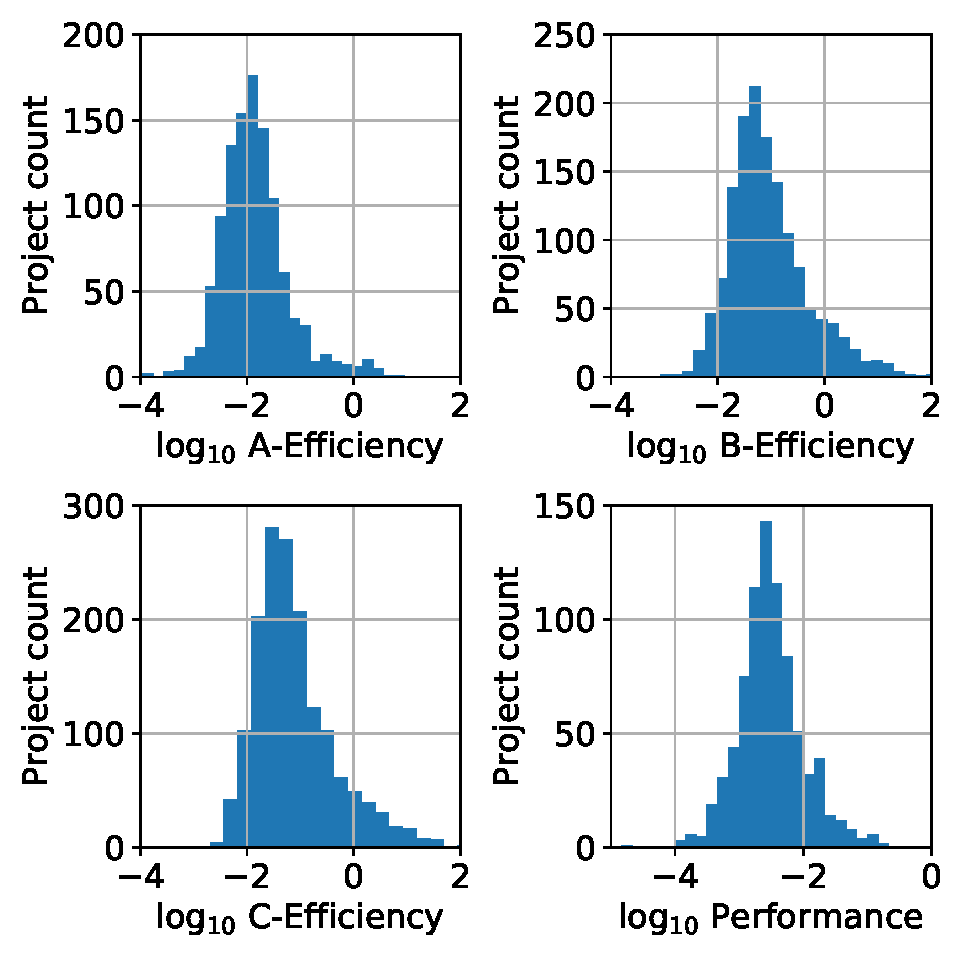
\includegraphics[width=2.5in,height=2.5in]{fig/WPProdPerf/fig-eff-perf-hist.pdf}
\caption{
Histograms of WikiProject productivity and performance.
Both measures are highly right-skewed, but form unimodal distributions
with low skewness after log transformation.
\label{fig:eff-perf-hist}
}
\end{figure}

\subsection{Empirical Results}

We find that both productivity and performance are highly right-skewed,
with a small number of projects having values much higher than the average.
After log-transforming the values, both the productivity and the performance have
a unimodal distribution with low skew (see Figure \ref{fig:eff-perf-hist}).
Our findings confirm the trade-off between performance and productivity
observed in many other settings (Figure \ref{fig:eff-perf}).
However, when looking at specific projects, some are higher in both performance
and productivity,
suggesting the existence of factors which correlate positively with both.

We also find that mean min-cut is highly correlated with degree ($r=0.980$, $p<0.001$),
so we exclude min-cut from regression models to prevent collinearity.
The high correlation between mean degree and min-cut implies that,
in most cases,
the minimum $st$-cut is simply the set of edges from $s$
or the set of edges to $t$.
The rarity of non-trivial min-cuts suggests that WikiProject coeditor
networks have very few central
bottlenecks and are thus highly decentralized.

\begin{figure}[t!]
\centering
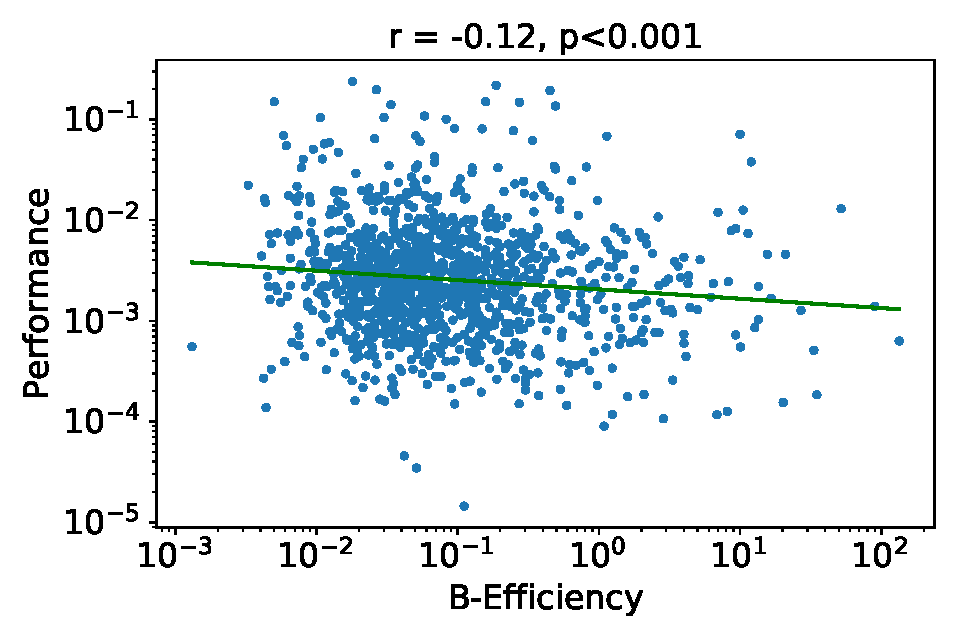
\includegraphics[width=2.5in,height=1.67in]{fig/WPProdPerf/fig-perf-eff.pdf}
\caption{
WikiProject performance is anticorrelated with B-level productivity,
with Pearson r of -0.12.
Results are similar for other grade levels.
On average, highly productive WikiProjects are under-performing,
but when looking at specific WikiProjects,
some are higher than others in both performance and productivity.
\label{fig:eff-perf}
}
\end{figure}

%\begin{figure}
%\centering
%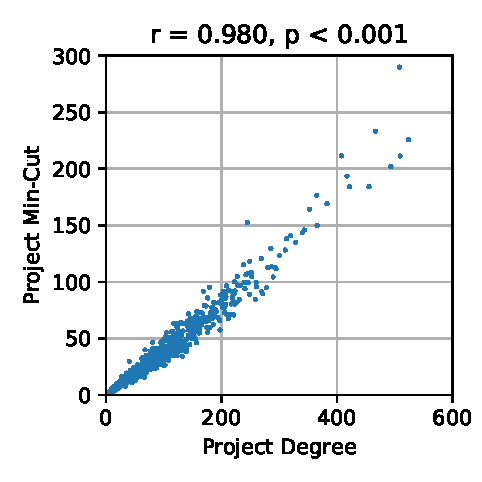
\includegraphics[width=2.33in,height=2.33in]{fig/WPProdPerf/fig-degree-mincut.pdf}
%\caption{
%Min-cut of WikiProject coeditor networks vs. their mean degree.
%\label{fig:degree-mincut}
%}
%\end{figure}

\begin{table}
\small
\begin{tabular}{lllllllll}
&Perf$^\dagger$&A-Eff$^\dagger$&B-Eff$^\dagger$&C-Eff$^\dagger$\\
\hline
Mean degree$^\dagger$&-0.7$^{***}$&-0.8$^{***}$&-0.6$^{***}$&-0.3$^{*}$\\
Out degree skew$^\dagger$&-0.4$^{***}$&-0.5$^{**}$&-0.3$^{*}$&-0.06\\
Mean path length$^\dagger$&-0.33$^{***}$&-0.09&-0.05&-0.09\\
C-productivity$^\dagger$&-0.08$^{*}$&\+---&\+---&\+---\\
Connected frac.&0.01&0.09$^{*}$&0.15$^{***}$&0.06\\
Talk fraction$^\dagger$&0&-0.02&-0.03&0.01\\
Mean similarity$^\dagger$&0.06$^{**}$&-0.03&0.01&0.02\\
Mean editors/art.$^\dagger$&0.3$^{**}$&0.3&0.2$^{*}$&0.09\\
Article count$^\dagger$&-0.4&0.7$^{*}$&0.8$^{**}$&0.7$^{**}$\\
Editor count$^\dagger$&0.4&0.9$^{**}$&0.8$^{**}$&0.5$^{*}$\\
Revision count$^\dagger$&0.6$^{*}$&-1$^{**}$&-1.1$^{***}$&-1$^{***}$\\
First assessment&0.05&0.11$^{**}$&0.31$^{***}$&0.43$^{***}$\\
Mean article age&-0.03&-0.04&-0.01&-0.05$^{*}$\\
\hline
N&1179&966&1260&1415\\
R$^2_{adj}$&0.37&0.17&0.30&0.43\\
\hline
\end{tabular}
\begin{tablenotes}
\item $\dagger$ Log-transformed. * $p < 0.05$. ** $p < 0.01$. *** $p < 0.001$.
\end{tablenotes}
\caption{Standardized coefficients for OLS models.
\label{tab:model}
}
\end{table}

To study the relationship between network structure, productivity, and performance,
we model the performance and productivity of WikiProjects using ordinary least-squares linear regression.
Each WikiProject is a single observation.
The models include each project's coeditor network properties as independent variables.
We also include the following project-level variables to control for confounding factors.
\begin{description}
\setlength\itemsep{0pt}
\item[C-productivity]
(performance only).
Quantifies how quickly a WikiProject improves articles.
Efficiencies for different grades are highly correlated,
so we include only one.
\item[Connected fraction.]
Fraction of coeditor pairs connected by a path.
\item[Talk fraction.] Fraction of total revisions made to talk pages.
\item[Mean similarity.] Mean Jaccard similarity (by article) with other WikiProjects; a measure of topical complexity.
\item[Mean editors/article.] Mean number of editors collaborating on each article in a WikiProject.
\item[Article count.] Total number of articles in the WikiProject.
\item[Editor count.] Total number of editors working on articles within a WikiProject.
\item[Revision count.] Total number of revisions to articles in a WikiProject.
\item[First assessment.] Timestamp of first assessment; a measure of how long a WikiProject has been active.
\item[Mean article age.] Mean age of articles within a WikiProject.
\end{description}

Our models are summarized in Table \ref{tab:model}.
Min-cut is excluded from all models to avoid collinearity,
as it is highly correlated with degree.
In-degree and out-degree skewness were also highly correlated,
so we only include out-degree skewness
(results are similar for in-degree skewness).
Heavy-tailed variables are log-transformed.
To test the robustness of our results,
we also computed models using cube root instead of logarithmic transformations,
and using only top- and high-importance articles.
The results were qualitatively similar results for all variables,
except for degree-skewness, which had an inconsistent sign across models.

We see that B-productivity and C-productivity have very similar models, but that A-productivity behaves
differently in its dependence on degree skewness and connectivity.
The different behavior of A-productivity is likely explained by the
observation that the A-Class quality is infrequently used in practice.
The A-Class quality level is usually passed when an article reaches
good or featured article status,
which follow deifferent a consensus process from other ratings.

The negative dependence of performance on C-productivity suggests there is generally a trade-off between
performance and productivity.
However, low degree is correlated with both higher productivity and higher performance,
suggesting that it is possible to improve both simultaneously.
Much of the existing numerical work on networked social learning focuses on path length rather than degree,
so we explore this result further using simulations in the next section.

For path length, we find that longer lengths correspond to lower performance, contrary to the conjecture
that longer path lengths allow more exploration \cite{mason_propagation_2008}
but consistent with a conformity-based social learning strategy \cite{barkoczi_social_2016}.

We also observe that high degree skewness is correlated with lower performance and lower A-productivity,
suggesting that projects with decentralized coeditor networks produce featured or good status
articles more quickly, and reach higher quality ratings in general.

\section{Agent-Based Model}
\label{sec:sim}

\begin{table*}[!ht]
\small
\centering
\begin{tabular}{lccccc}
Name          & Social stage & Individual stage & Limited concern & Unknown objective & Single truth \\
\hline
Best+I & Best neighbor   & Global & & & \\
Conf+I & Conformity      & Global & & \Checkmark & \\
Best+LI & Best neighbor  & Local  & \Checkmark & & \\
Conf+LI & Conformity     & Local  & \Checkmark & \Checkmark & \\
LMaj+LI & Local majority & Local  & \Checkmark & \Checkmark & \Checkmark \\
\hline
\end{tabular}
\caption{
Definitions and properties of social learning strategies.
Each consists of a social stage and an individual stage.
Individual stages use hill-climbing based on either the global state,
or the agent's local concern.
\label{tab:strat}
}
\end{table*}

In addition to our empirical study,
we use a simple agent-based model of collaboration to better understand
the relationship between node degree, productivity, and performance.
Numerical models allow us to determine the effect of changing a single
variable (e.g., network structure, learning strategy),
which is impractical in the empirical setting.
It is important to note that the goal of our model is not to simulate
all the intricacies of Wikipedia or any other specific platform.
Rather, our goal is to determine whether the correlations we observe
between degree and outcome variables
on Wikipedia can be reproduced in a more general setting.

Past work in the field of social learning typically models collaboration
as an optimization problem:
finding a state of the world which maximizes some objective function
\cite{lazer_network_2007,mason_propagation_2008,mason_collaborative_2012,barkoczi_social_2016}.
Wikipedia itself can be regarded as an optimization problem.
On Wikipedia, editors are generally seeking to improve the quality of articles
and have some personal preference over possible states of an article.
When editors do not agree on the optimal state of an article,
the conflict is resolved through a consensus-based deliberation.
This consensus process can be regarded as a {\em social choice function}
\cite{arrow_social_2012,brandt_computational_2012}
which maps individual preferences to community preferences.
Wikipedia can thus be thought of as a group of editors with individual preferences
for article states,
collaborating to optimize articles according to community preferences.
Note that these community preferences do not assume the existence of any
ground truth, other than the preferences themselves.

To simulate collaboration, we need a model problem for collaborators to solve.
Following existing literature on social learning,
we use the NK model \cite{kauffman_towards_1987}
to create NP-hard, nonlinear optimization problems.
The NK model produces an objective function with a
{\em rugged landscape}, i.e., many local optima.
The ruggedness of the model can be tuned through the parameters $N$
(the dimensionality of the solution space)
and $K$ (the level of inderdependence between dimensions).
Formally, the NK model produces an objective function $F$ mapping a binary string $S$ of length
$N$ to a real value in $[0,1]$.
Model state is divided into $N$ {\em loci}, with locus $i$ having a binary state $S_i$
and a value $f_i(S)$ dependent on its own state
and on the state of $K$ random other loci.
The functions $f_i(S)$ are created by selecting a random value in $[0,1]$ for
each possible state of locus $i$ and its $K$ neighbors.
The value of the model $F(S)$ is the mean of all locus values $f_i(S)$.
In our simulations,
agents iteratively search for a bit string $S$ that maximizes $F(S)$.

In a typical social learning model,
a set of agents each maintain an estimate of the optimal state
and iteratively update that estimate based on information available from other agents,
according to some {\em learning strategy}.
In networked social learning,
agents are associated with the nodes of a network and share information
only with their neighbors.
We define productivity and performance in terms of the solution values for each time step
(averaged over many trials).
We define the performance to be the mean solution value after the process has converged,
while the productivity is the reciprocal of the number of steps required to converge.
We measure the time to convergence as the number of steps required to reach 99\% of the maximum
mean solution value.

Without additional constraints,
the above model is missing
several key properties of real-world collaborations.
In designing our agent-based model, we paid attention to the
following properties.
\begin{description}
\setlength\itemsep{0pt}
\item[Limited concern.] Agents are concerned only with a subset of the entire
state when making decisions and determining preferences.
(On Wikipedia, editors typically interact with a small subset of the articles.)
\item[Concern-based network.] Agents interact with other agents who share a
common concern over some subset of the state.
(On Wikipedia, editors interact with others who share interests in the same articles.)
\item[Unknown objective.] Agents rank states in order of preference,
but do not have access to the objective function.
(On Wikipedia, there is no ground truth measure of quality.)
\item[Single source of truth.] At any given time, the system is in a single state
and agent preferences are based on local modifications to that state.
(At any point in time, there is only one current version of Wikipedia.)
\end{description}

\subsection{Concern-Based Networks}

On Wikipedia, editors interact by editing articles and talk pages.
Thus, the editors who interact with each other are exactly those who care about the same content.
Rather than using arbitrary networks,
we devise a network structure inspired by the above observation.
We do so by associating agents with particular loci in the NK model.
We also wish to study the effect of varying network degree,
which we achieve through a rewiring process described below.

Our concern-based networks are generated directly from the structure of the NK model.
The value of each NK locus depends on its own state and the state of $K$ other loci.
For each locus, we define an agent and assign these $K+1$ loci as its concern.
Next, an agent-agent co-affiliation network is created by connecting two agents if they share at least
one locus in their concerns.
This process is analogous to our construction of WikiProject coeditor networks.

To create a tunable degree, we duplicate each agent and its concern,
then randomly rewire a fraction of agent concerns before creating the agent-agent network.
With no rewiring, the duplication process creates a high overlap between agent concerns.
This overlap results in redundant links to a small number of agents,
rather than unique links to a large number of agents,
and therefore to an agent-agent network with small average degree.
By randomly rewiring the agent concerns, the redundancy is reduced
and the average degree of the agent-agent network is increased.

\subsection{Networked Learning Strategies}

Learning strategies determine how agents update their preferences based on
available information \cite{barkoczi_social_2016}.
Agents can engage in individual learning
by applying a hill-climbing algorithm to their current solution.
In each iteration, one bit of the NK solution string is flipped to maximize the solution value.
If no change improves the value, the original solution is kept.
The above strategy relies only on rankings of states,
satisfying the unknown objective assumption.
However, it relies on information about the entire state,
violating the limited concern assumption.
In order to satisfy this assumption,
we also define a local variant
in which only a subset of bits in the NK solution string are considered.
This variant reflects a more realistic style of collaboration,
in which individual agents focus on sub-problems.

In social learning,
agents can also incorporate information from
other agents they are connected to by an edge.
While individual learning always converges to the local maximum relative to the starting point,
social learning strategies allow agents to ``jump'' to drastically different solutions with higher local maxima.
In our model, we use both the conformity and best-neighbor strategies from \cite{barkoczi_social_2016}.
In the {\em best-neighbor} strategy, each agent compares its solution to a sample of neighbors, and chooses the solution with the highest value.
In order to compare solutions between neighbors,
the exact value of the objective function must be known for each solution,
so this strategy does not satisfy the unknown objective assumption
or the limited concern assumption.
In the {\em conformity} strategy, agents simply choose the most common solution among their neighbors
(ties are broken uniformly at random).
This strategy does not rely on solution value at all, so clearly satisfies the
unknown objective and limited concern assumptions.
In both cases, a single iteration of individual learning is performed after each social learning
iteration.
Because each agent maintains a separate estimate of the solution,
neither strategy satisfies the single source of truth assumption.

\subsection{Local Majority Strategy}

To satisfy the single source of truth assumption,
we introduce a new strategy: {\em local majority}.
In local majority, agents all begin with the same starting state and apply individual learning to their concern to generate
possible improvements to the solution.
Next, a new solution is constructed by considering each locus of the NK solution
individually.
Every agent concerned with a locus votes for its state based on their preferred
new solution and the majority state is chosen.
The result of this process is that all agents integrate their solutions into
a single state,
which forms the basis for the next iteration.
This strategy more realistically reflects collaborations like Wikipedia:
at any given time, a Wikipedia article has a single state, determined by consensus,
but editors may have differing opinions on how to improve that article.

\subsection{Simulation results}

We simulated 100 trials for rewiring values of 0.0, 0.167, 0.333, 0.5, 0.667, 0.833, and 1.0.
For each trial we generated an NK model with $N=250$ and $K=7$,
generated a concern-based network, and ran each social learning strategy
(Table \ref{tab:strat}) for 300 iterations.
For conformity and best-neighbor strategy, we used a sample size of 3, following
\cite{barkoczi_social_2016}.
We confirmed that all trials converged to their maximum value before reaching
the last iteration.
Networks had mean degree 116.6 with 1.3 standard deviation,
and mean path length of 1.766 with 0.0027 standard deviation.
The coefficient of variation for degree is approximately 10\%,
while only 1\% for mean path length, confirming that the rewiring process has a stronger influence
on degree than on path length.

\begin{figure}[t!]
\centering
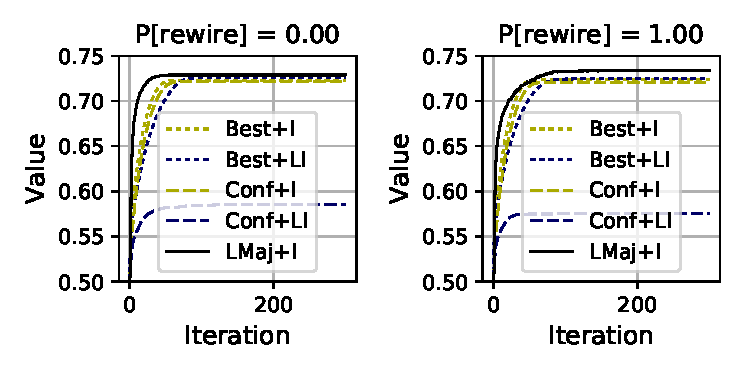
\includegraphics[width=3in,height=1.5in]{fig/WPProdPerf/fig-val-iter.pdf}
\caption{
Mean agent solution value over time, averaged over 100 trials.
Strategies are defined in Table \ref{tab:strat}.
\label{fig:val-iter}
}
\end{figure}

\begin{table}
\small
\centering
\begin{tabular}{lll}
Strategy & Performance & productivity\\
\hline
Best+I  & 0.722 $\pm$ 0.001 & 0.0221 $\pm$ 0.0003 \\
Conf+I  & 0.721 $\pm$ 0.001 & 0.0174 $\pm$ 0.0002 \\
Best+LI & 0.726 $\pm$ 0.001 & 0.0131 $\pm$ 0.0002 \\
Conf+LI & 0.586 $\pm$ 0.001 & 0.030 $\pm$ 0.001 \\
LMaj+LI & 0.729 $\pm$ 0.001 & 0.046 $\pm$ 0.002 \\
\hline
\end{tabular}
\caption{
Simulated Performance and productivity.
Results shown for 100 trials with P[rewire] = 0.
Strategies are defined in Table \ref{tab:strat}.
Local strategies are less productive than their non-local counterparts.
Local best-neighbor out-performs global,
while local conformity is the worst performer in all cases.
The local majority strategy is both most productive and most performant.
\label{tab:sim-eff-perf}
}
\end{table}

\begin{table}
\small
\centering
\begin{tabular}{lll}
Strategy & Perf. Std. Coeff. & Eff. Std. Coeff.\\
\hline
Best+I  & -4.2$\times{10^{-5}}$ & \+4.1$\times{10^{-5}}$ \\
Conf+I  & \+2.7$\times{10^{-5}}$ & \+9.4$\times{10^{-5}}$ \\
Best+LI & -9.6$\times{10^{-4\;**}}$ & \+7.7$\times{10^{-5}}$ \\
Conf+LI & -1.5$\times{10^{-3\;***}}$ & \+8.7$\times{10^{-5\;*}}$ \\
LMaj+LI & \+1.2$\times{10^{-4\;**}}$ & -0.038$^{***}$ \\
\hline
\end{tabular}
\begin{tablenotes}
\item \centering * $p < 0.05$. ** $p < 0.01$. *** $p < 0.001$.
\end{tablenotes}
\caption{
Degree regression coefficients for simulations.
\label{tab:sim-perf}
}
\end{table}

\begin{figure*}
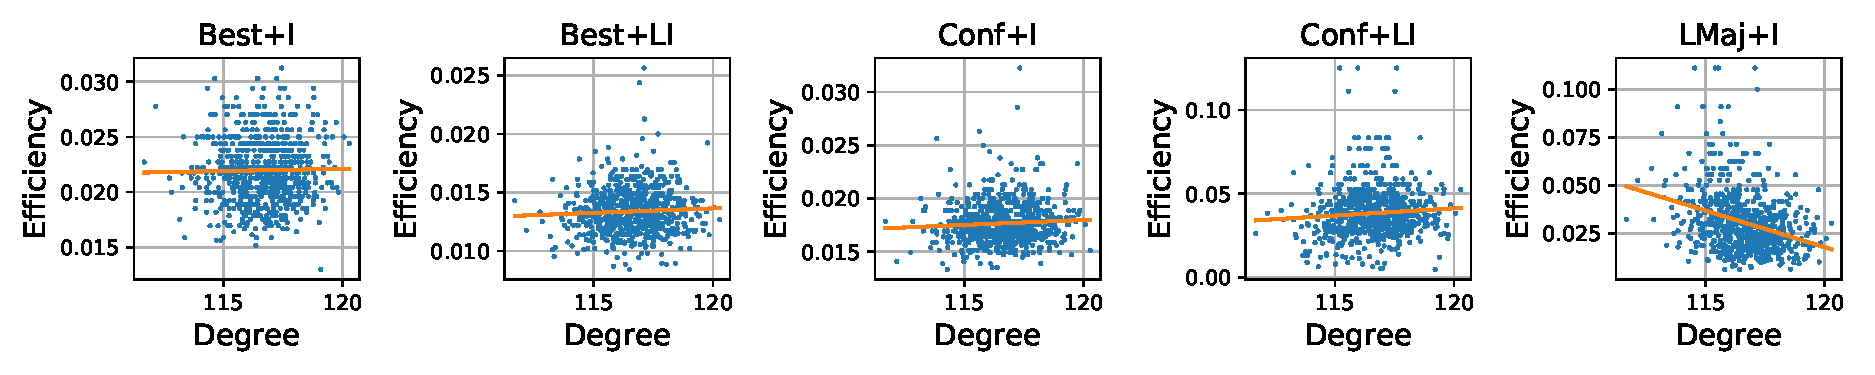
\includegraphics[width=6.67in,height=1.33in]{fig/WPProdPerf/fig-deg-eff.pdf}
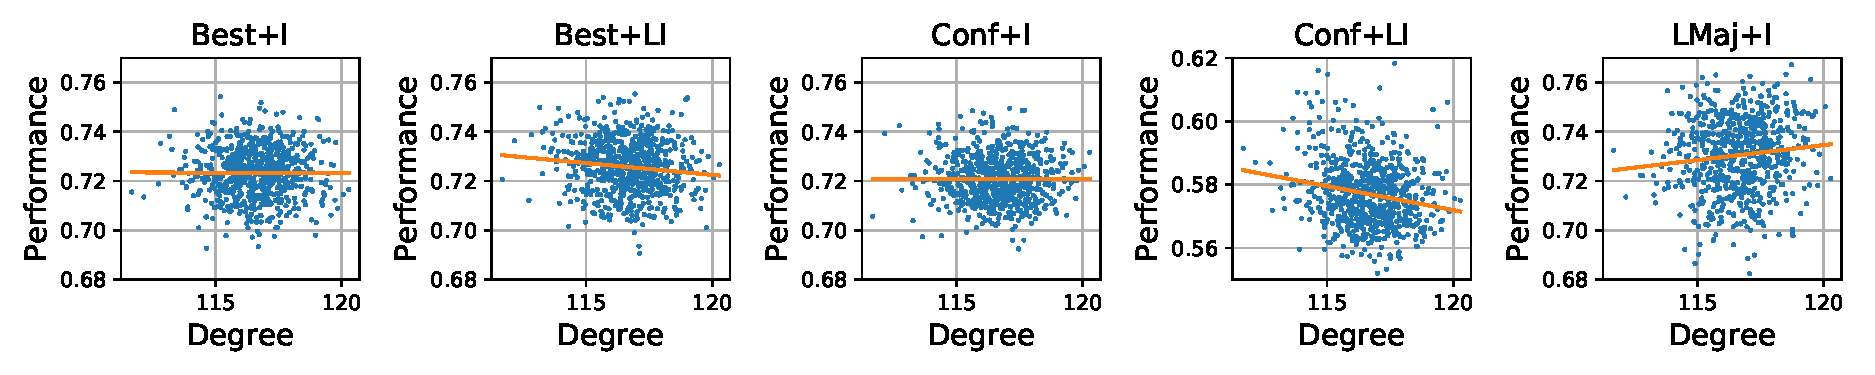
\includegraphics[width=6.67in,height=1.33in]{fig/WPProdPerf/fig-deg-perf.pdf}
\caption{
productivity and Performance of social learning strategies vs. mean network degree.
Each point represents a single trial of 300 iterations.
Strategies are defined in Table \ref{tab:strat}.
The local best-neighbor strategy shows
decreased performance at high degree,
with no significant change in productivity.
Local conformity shows decreased performance and increased productivity at high
degree.
Local majority shows the opposite behavior:
increased performance and decreased productivity at high degree,
with the productivity showing the largest effect size of all strategies.
\label{fig:deg-eff-perf}
}
\end{figure*}

Figure \ref{fig:val-iter} shows how agents' solutions improve after repeated applications of
different learning strategies and rewiring values.
Each curve represents an average over 100 trials, each with 250 agents.
The mean performance and productivity are reported in Table \ref{tab:sim-eff-perf}.
For all rewiring values, local strategies are less productive and more performant
than their non-local counterparts.
For the best-neighbor strategy, local outperforms global.
Local conformity performs notably worse than all others.
Local majority is both more productive and more performant than others,
with its performance increasing with higher rewiring.
This implies that,
at least in a simple collaboration model,
performance and productivity can be simultaneously increased.
Furthermore, performance and productivity are potentially affected by both the choice of
learning strategy and the average degree of the agents' social network.

The effects of degree on performance and productivity are shown in Figure \ref{fig:deg-eff-perf} and
Table \ref{tab:sim-perf}.
For non-local versions of both conformity and best-neighbor strategy,
there is no significant effect of degree on performance or productivity.
The local best-neighbor strategy shows reduced performance with increasing degree,
but no change in productivity.
Local conformity and local majority show opposite behavior as degree increases:
with local conformity gaining productivity at the expense of performance,
while local majority increases in performance and decreases in productivity.
The largest effect size is achieved for productivity in the local majority simulation,
which is consistent with the productivity behavior observed in WikiProjects.
However, the performance behavior for local majority is opposite that observed on
Wikipedia.
These agent-based models confirm that network degree has the potential to influence
the performance and productivity of collaborations.
Furthermore, this influence can be drastically different depending on the strategies
used by collaborators.

\section{Discussion}
\label{sec:discuss}

While existing research into the role of network structure in collaboration
has focused on numerical simulations and lab experiments,
analysis of large real-world systems is an important next step.
Our empirical analysis contributes several findings towards a better
understanding of large, decentralized, real-world collaboration.
We observe several results consistent with previous work:
a trade-off between performance and productivity
\cite{mason_propagation_2008,grim_scientific_2013},
higher performance for shorter path lengths in a conformity setting
\cite{barkoczi_social_2016},
and a reduction in performance with increased structural inequality
\cite{kearns_experiments_2012}.
By using real-world networks, we were also able to analyze network properties independently.
While most existing work has focused on the importance of path length,
our findings suggest degree distribution may be just as, or more, important.
The association of low degree with both high performance and high productivity is compelling,
as it sidesteps the usual trade-off between performance and productivity.
In low-degree networks, agents have more repeated interactions with smaller groups of collaborators, suggesting that small team sizes could be beneficial for large collaborations.
Similarly, the observation that performance is higher in projects with less structural inequality suggests that,
if the challenges of egalitarian organizing are overcome,
decentralized collaborations may produce better outcomes than those with centralized, top-down structures.

Our agent-based models offer a several insights.
We observe degree-dependent performance and productivity
for both local conformity and local majority strategies.
However, these two strategies have opposite degree dependence,
suggesting that different strategies may be preferable for high-degree and low-degree
networks.
Our local majority strategy,
designed to satisfy several properties found in real-world collaborations,
shows the strongest effects on performance and productivity as network degree changes.
For the local majority strategy,
the relationship between degree and productivity is consistent with our
empirical observations on Wikipedia,
suggesting one possible mechanism underlying that productivity dependence.
However, the performance dependence of this strategy
is opposite that observed on Wikipedia,
suggesting that either the local majority strategy
is incompatible with actual behavior on Wikipedia or
that other factors outweigh the contribution of mean degree.

Our work has several limitations.
Our empirical analysis is purely correlative and cannot be used to draw
conclusions about the causal influence of network structure on collaboration.
However, the consistency of our results with other lab-based and numerical studies
suggests that the causal link is worthy of further study.
Similarly, our study focuses entirely on a single online community,
and while the results are suggestive, they do not necessarily generalize.
We have focused on structure, ignoring content-related variables.
For simplicity, we have assumed unweighted edges and
measured work by revision counts rather than bytes changed.

Our work suggests several directions for future work.
Is the correlation between network structure, performance, and productivity causal?
A time-dependent analysis of our data could offer insight.
Are similar relationships observed in other large-scale collaborations?
Does varying degree independently of path length influence
performance and productivity in a controlled lab setting?

A better understanding of the relationship between network structure and collaboration
outcomes has practical applications.
Online communities using recommender systems could make recommendations guided by desirable network properties.
Similarly, network structure could be used to identify under-performing
groups in need of an intervention.
The relationship between network structure and learning strategy suggests that
behaviors interact with network structure,
which could be used to encourage behaviors complementary to existing network
structure.

\section{Conclusion}
\label{sec:conclusion}

In this paper, we have described the relationship between the structural properties of WikiProject
coeditor networks, their performance, and their productivity.
As in other studies, we see a trade-off between performance and productivity.
However, 
some properties, such as low degree, are associated with
both higher performance and higher productivity.
We also find that the correlations between path length and performance are consistent with a conformity-based
social learning strategy, but not a greedy best-neighbor strategy.
We observe improved performance in more decentralized projects,
as has been seen in small-scale lab experiments.
We have also proposed a novel local majority learning strategy that is more realistic,
more productive, and higher performance than existing strategies.
While most previous social learning simulations focus on path length,
we observe degree-dependent performance and productivity
in both the local majority strategy
and a localized version of the conformity strategy.
We find that the direction of that dependence varies with the
specific strategy being used.
While additional work is needed to determine causal relationships
and the generalizability of our results,
we have shown evidence that several phenomena predicted by numerical
and small-scale lab experiments are present in a large,
real-world collaboration.
Our results suggest that the success of large-scale collaborations may be aided
by greater decentralization,
consensus or conformity-based decision-making,
and more tightly-knit collaborations between smaller teams.



\chapter{Small interlocking groups improve mass deliberation in the presence
of strong social influence}
\label{chap:abm}
\section{Introduction}

Deliberation enables the generation, aggregation, and synthesis of diverse knowledge \cite{dewey_creative_1940, anderson_epistemology_2006, ackerman_deliberation_2002, ostrom_collective_2000},
as well as the early identification and resolution of conflict \cite{gentry_consensus_1982}.
As a participatory process, deliberation builds trust among participants, increases the perception of fairness, and incentivises cooperation with group decisions
\cite{ostrom_collective_2000, bowles_endogenous_1998}.
As a dynamic process, deliberation alters private preferences through discourse \cite{habermas_structural_1991}, sidestepping fundamental limitations of voting, e.g., the Condorcet paradox \cite{condorcet_essay_1785, brandt_computational_2012} and Arrow's impossibility theorem \cite{arrow_social_2012, brandt_computational_2012}.
Despite these benefits, deliberation becomes prohibitively difficult in larger groups, due to the increased time and effort needed to reach decisions \cite{fishkin_voice_1997, gentry_consensus_1982} and to the emergence of power inequalities \cite{freeman_tyranny_1972, boehm_egalitarian_1993}.
Yet examples of successful mass deliberation do exist, including Wikipedia \cite{giles_internet_2005, keegan_evolution_2017}, free and open source software projects \cite{benkler_coases_2002}, grassroots protest and crisis-response networks \cite{gonzalez-bailon_networked_2016, brugh_combining_2019} and self-managed organizations \cite{laloux_reinventing_2014}.
The commonalities between such projects provide insight into overcoming the challenges of mass deliberation.
Specifically, we evaluate a model of mass deliberation inspired by common network features observed in successful projects.

Communication in large collaborations is necessarily restricted when group size exceeds individual members' capacity for communication. The structure of the resulting communication network is an important factor in the success of collaborative tasks \cite{kearns_experiments_2012, mason_collaborative_2012, mason_propagation_2008}, such as deliberation. Among successful mass deliberative projects, communication networks often exhibits a common structure: small interlocking groups \cite{benkler_coases_2002, gonzalez-bailon_networked_2016, brugh_combining_2019, laloux_reinventing_2014}. A similar structure has been observed in the interlocking directorates of corporate boards \cite{karau_social_1993} and the interlocking publics of the public sphere \cite{habermas_structural_1991}, as well as utilized for collective design in network rotation \cite{salehi_hive_2018}.
These interlocking groups have been given various names: committees, working groups, projects, modules, affinity groups, circles, teams, cores, nodes, zones, cells, or syndicates.
We shall use the term {\em pods} to encompass all groups exhibiting two key characteristics: small enough to enable deliberation, and interlocking to enable information diffusion.
We shall use the term {\em network deliberation} to refer to mass deliberation using an interlocking pod structure.
Communication network structure also influences the success of collaborations by controlling the speed of information diffusion \cite{lazer_network_2007,mason_propagation_2008,mason_collaborative_2012,barkoczi_social_2016, gomez_clustering_2019,derex_partial_2016,kearns_experiments_2012}. Structurally efficient networks enable fast diffusion and favor exploitation of known information over exploration of the unknown \cite{lazer_network_2007, barkoczi_social_2016}. In the context of network deliberation, structural efficiency is determined by how individuals are assigned to pods.
We will focus on two such methods: one efficient, one inefficient.

Collective tasks such as deliberation are influenced not only by communication structure, but also by individual behavior. Individuals weigh social influence against their personal knowledge and expertise  \cite{boyd_culture_1988}. 
Even in a collective setting, individuals sometimes work independently to search for new and innovative ideas \cite{lazer_network_2007, barkoczi_social_2016}, to utilize their unique information and perspectives \cite{hong_interpreted_2009}, and to critically evaluate the ideas of others \cite{rendell_rogersparadox_2010}.
Alternatively, individuals can defer to others in order to exploit and propagate good ideas \cite{barkoczi_social_2016, boyd_culture_1988}, to conserve their own resources through free-riding and social loafing \cite{karau_social_1993}, or due to a high level of trust \cite{salehi_hive_2018} or social influence \cite{banerjee_simple_1992, smith_pathological_2000}. Individual behavior interacts with network structure to vary the level of exploration of new ideas versus the exploitation of known information \cite{barkoczi_social_2016}. While the focus of network deliberation is structural, the effect of network structure must be understood in the context of individual behavior and social dynamics.

We model network deliberation using a social learning framework to address two questions. How effective is network deliberation compared to conventional single-group deliberation? And how do network efficiency and individual behavior influence the outcome of network deliberation? We present the following three contributions.
First, network deliberation out-performs conventional deliberation in both solution speed and quality when agents rely heavily on social learning. This suggests that network deliberation is a promising deliberation design for groups with a high degree of social influence. Second, network deliberation performs best on structurally efficient networks when agents exhibit conformist behavior, while it performs best on structurally inefficient networks when agents greedily maximize solution quality, consistent with findings for conventional networks \cite{barkoczi_social_2016}.
Third, the naive greedy strategy can be modified to improve performance on conventional networks despite using strictly less information. In the case of network deliberation, the naive and modified greedy strategies are equivalent.

\section{Methods}

Deliberation can be modeled as a form of collective problem-solving and social learning in which agents hold private beliefs, share information with their neighbors, and update their beliefs based on a combination of individual analysis and social influence.
Following existing models of collective problem-solving \cite{lazer_network_2007, barkoczi_social_2016, gomez_clustering_2019}, our model comprises: 1. a collective task, 2. a network, and 3. a learning strategy.
Agents maintain a candidate solution to the task and iteratively apply their learning strategy to the available information, yielding an updated candidate.

\subsection{Overview}

As their collective task, agents seek an optimal point on a rugged fitness landscape.
This landscape is generated using the NK model \cite{kauffman_towards_1987, weinberger_local_1991} (see Appendix \ref{apx-nk}).
The NK model is a ``tuanbly rugged'' objective function parameterized by two variables:
the number of bits in the input string ($N$),
and the number bits used to compute each contribution to the objective function ($K+1$).
These parameters can be used to tune problem size and complexity, respectively.
The resulting objective function maps $N$-bit strings to real numbers in $[0,1]$.

To model network deliberation, we construct interlocking networks in stages. At each stage, agents are partitioned into small {\em pods} and connected to all other agents in the same pod.
Our choice of pod size is informed by real-world The upper limit of effective small group size has been estimated variously as five \cite{freeman_tyranny_1972}, five--eight\cite{lohman_designing_2000}, and eight \cite{miflin_small_2004}.
We choose a pod size of 5.
Different methods for assigning agents to pods produce networks with different properties.
Interlocking structure is created when agents are placed with others they have not yet interacted with.
We thus require that pod assignment methods satisfy the following mixing property:
\begin{property}
\label{prop:mixing}
For any agent $v$, and any two assignment stages $t$, $t^\prime$, the probability that at least one neighbor of $v$ at stage $t$ is also a neighbor at stage $t^\prime$ approaches 0 as $|V|$ grows.
\end{property}
We study two such methods: a random assignment method that produces structurally efficient networks, and a long-path method that produces inefficient networks. For comparison, we also simulate conventional deliberation. While the potential communication links in conventional deliberation form a fully connected network, actual communication is better modeled by preferential attachment \cite{barabasi_emergence_1999} or small-world \cite{watts_collective_1998} networks (see Methods).

An agent's learning strategy models both informational constraints and behavioral dynamics \cite{lazer_network_2007, barkoczi_social_2016} such as social influence and social loafing \cite{karau_social_1993}.
We consider three social learning strategies.
The {\em best-neighbor} strategy is the naive greedy strategy: agents simply adopt the neighboring solution with the highest value. This strategy requires that agents have the ability to compare the quality of two arbitrary solutions, a strong assumption representing either skilled agents, or a simple task.
The {\em conform} strategy is pure social influence. Agents adopt the most common solution among their neighbors.
This strategy requires no knowledge of solution quality, modeling contexts where agents are unable to compare solution quality, or where agents choose not to, as in social loafing \cite{karau_social_1993}.
We also introduce the {\em confident-neighbor} strategy, a variant of best-neighbor in which agents announce when they have the best solution in their neighborhood. This variant makes weaker assumptions about agent ability but is equivalent to best-neighbor when network deliberation is used.
This strategy allows us to compare low-social influence and high-social influence strategies under equivalent assumptions of agent ability.

Between each stage of social learning, agents may perform individual learning. Following existing literature \cite{lazer_network_2007, barkoczi_social_2016}, we model individual learning by mutating a single bit of an agent's solution, and keeping it if the mutation improves solution quality.
A complete learning strategy must also specify how social and individual learning are integrated. Existing literature \cite{lazer_network_2007, barkoczi_social_2016} applies individual learning only when social learning fails to produce an improved solution. We refer to this method as {\em fallback} individual learning. Fallback can be also be interpreted as a model of social loafing \cite{karau_social_1993}. For completeness, we include analysis for a second method in which agents first perform social and individual learning in {\em parallel} and then choose the better of the two learning outputs.

\subsection{Agent-Based Model}

We use an agent-based simualation to model deliberation between individuals.
We model communication between agents using a time-dependent network $(V,E_t)$.
The vertices $V$ correspond to the agents (individuals).
The edges $E_t$ allow agents to exchange information with their immediate neighbors at time $t$.
Over the course of the simulation, agents seek to maximize some objective function $Q(s)$.
We use binary strings of length $d$ as our solution space: $s \in \mathbb{Z}^d$.
We generate the objective function $Q(s)$ using the NK model \cite{kauffman_towards_1987, weinberger_local_1991} (see Appendix \ref{apx-nk}).

The simulation begins at time $t=0$ by generating a set of initial solutions $s_{v,0}$ for the agents.
These are generated randomly, with each possible solution having equal probability.
The simulation proceeds iteratively.
At time $t$ each agent applies one of several {\em learning strategies}, to determine its preferred solution at time $t+1$.
Learning strategies can rely on the agent's own solution, the solutions of its neighbors, and potentially additional information shared by its neighbors.
Learning strategies may also incorporate information about the objective function, modeling an agents' ability to evaluate the quality of solutions.
To allow for ties, learning strategies produce a set of solutions rather than a single solution.
In our simulations, we choose winners at random in the case of a tie.
We present results for 1000 randomly generated NK model objectives.
with each network/strategy combination simulated once per objective function.
In keeping with other authors \cite{barkoczi_social_2016, lazer_network_2007} we use $N=15$ and $K=6$.
We allow each simulation to proceed for 300 iterations, which we have found sufficient to guarantee convergence with our chosen parameters.

\subsection{Networks}

We carry out simulations for four different network topologies. In addition to the well-known preferential-attachment \cite{barabasi_emergence_1999} and small-world \cite{watts_collective_1998} networks, we construct two types of networks to model network deliberation.
Both types exhibit interlocking structure and satisfy Property \ref{prop:mixing}.
These two network deliberation conditions differ in how agents are assigned to pods and in the structural efficiency of the resulting network.
At each iteration, existing edges are replaced with cliques corresponding to the pods. An edge is created between two agents if and only if they share a pod.
In {\em random-pod} assignment, agents are assigned to pods at random.
This assignment method produces short geodesic paths and efficient network structure.
In {\em long-path} assignment, agents are assigned using an algorithm which guarantees interlocking structure while preventing the creation of long-distance ``shortcut'' edges, producing a structurally inefficient network.
All networks are constructed with 100 vertices/agents and a mean degree of 4 (pod size of 5).

\subsection{Conventional Deliberation}
We model the communication network structure of conventional deliberation using two static networks: small-world networks \cite{watts_collective_1998}, and preferential attachment networks \cite{barabasi_emergence_1999}. In typical deliberative settings, from deliberative assemblies to online forum threads, the contributions of any member are potentially visible to all other members.
The network of {\em potential} communication can be modelled by a complete graph.
However, a complete graph may not be the best model for the {\em actual} communication that takes place in such a network. In a real-world deliberation, some participants are more influential than others \cite{goel_structure_2012, shaw_laboratories_2014}, and many communications can be missed or ignored by any particular participant.

Human social networks often exhibit large clustering, and short path lengths.
To model such dynamics, we use Watts-Strogatz small-world networks  \cite{watts_collective_1998}.
These networks model, for example, when participants interact mostly with their strong ties, but occasionally with a weak tie. Social networks have also been found to exhibit skewed degree distributions with long tails \cite{barabasi_emergence_1999}.
We model these networks using the Barabási-Albert preferential attachment model.
These networks model settings where a small number of individuals produce a disproportionate share of the communication due to factors such as social capital, expertise, or confidence.

\subsection{Network Deliberation: Interlock Networks}
Both of our network deliberation conditions use networks built from interlocking pods.
These pods are small complete graphs of roughly equal size.
At any given time, each agent can communicate with all other agents in exactly one pod.
Periodically, all agents are simultaneously reassigned to new pods.
These reassignments create an interlocking structure, allowing information to flow through the entire group.
This structure can be represented as a time-dependent or directed network.
The properties of an interlock network depend on the particular method for assigning agents to pods.
Crucially, interlocking structure is created when agents are placed with others they have not yet interacted with.
We thus require that pod assignment schemes satisfy the mixing property (Property \ref{prop:mixing}).

\subsubsection{Random-Pod Assignment}
The {\em random-pod} assignment method (Algorithm \ref{alg:random}) simply assigns agents to groups at random. Pseudocode for this method is shown in Algorithm \ref{alg:random}.

\begin{algorithm}
\SetAlgoLined
\DontPrintSemicolon
\SetKwFunction{removeRandom}{removeRandom}
\SetKwFunction{insert}{insert}
\SetKwFunction{emp}{empty}
\SetKw{algnot}{not}
\KwData{A vertex list $V$, the pod size $M \in \mathbb{Z}$.}
\KwResult{A partition of the vertices.}
    $N \longleftarrow \lceil \frac{|V|}{M} \rceil$ \;
    $P \longleftarrow$ List of $N$ empty sets \;
    \For{$i \in 1, \ldots, M$}{
        \ForEach{$s \in P$}{
            \If{\algnot $V.\emp()$}{
                $v \longleftarrow V.\removeRandom()$ \;
                $s.\insert(v)$ \;
            }
        }
    }
    \Return{$P$}
\caption{Random-Pod Assignment}
\label{alg:random}
\end{algorithm}

\begin{claim}
Random-pod assignment satisfies Property \ref{prop:mixing}.
\end{claim}

\begin{proof}
Let $v$ be a vertex of graph $G=(V,E_t)$ with a set of $M$ neighbors at stage $t$ denoted $N_t(v)$.
The probability that the $k$th neighbor chosen at time $t^\prime \neq t$ belongs to $N_t(v)$, given that the first $k - 1$ did not, is:
\begin{align*}
p_\text{repeat}(k)
&= \frac{M - 1}{|V| - k} \\
&\leq \frac{M - 1}{|V| - M}.
\end{align*}
The probability that none of the $M-1$ neighbors chosen at time $t^\prime$ belong to $N(v)$ thus satisfies:
\begin{align*}
p_\text{mixed}
&\geq
\left( 1 - \frac{M - 1}{|V| - M} \right)^{M-1} \\
\lim_{|V|\rightarrow\infty} p_\text{mixed}
&= 1
&\qedhere
\end{align*}
\end{proof}

Random pod assignment also creates structurally efficient networks with short geodesic distances, as shown in Figure \ref{fig:broadcast}.
There has been evidence both for
\cite{lazer_network_2007, derex_partial_2016, mason_propagation_2008, barkoczi_social_2016}
and against
\cite{mason_collaborative_2012, barkoczi_social_2016}
the effectiveness of structurally efficient networks in social learning.

\begin{figure}
    \centering
    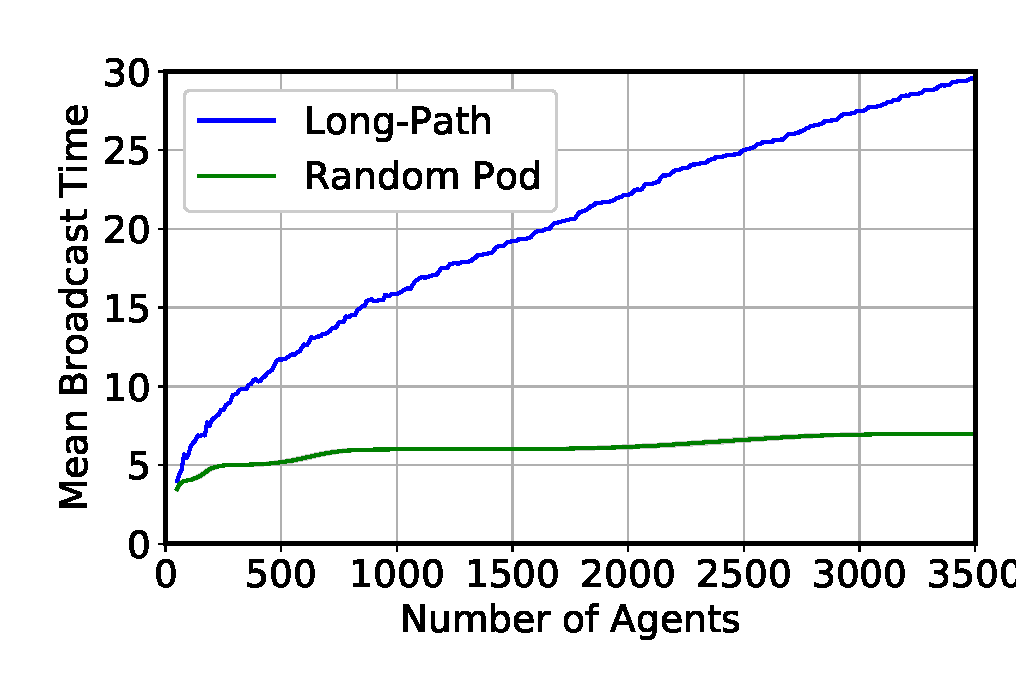
\includegraphics[width=3.33in]{fig/NetDelibABM/fig-broadcast.eps}
    \caption{Mean time necessary for a signal broadcast from one node to reach the entire network. We use mean broadcast time as a measure of geodesic length for time-varying networks.}
    \label{fig:broadcast}
\end{figure}


\subsubsection{Long-Path Pod Assignment}

To study the effects of path length, we require an alternative pod assignment method that produces long paths.
However, we must still retain Property \ref{prop:mixing} such that it is rare for two agents to repeatedly share the same pod.
This property ensures the creation of many new edges at each stage, which is difficult--but not impossible--to reconcile with long average path length.
We now present a {\em long-path} pod assignment method, which meets both of the above goals.

We begin with a high-level overview.
Agents are assigned an integer position on a 1-dimensional circular lattice.
By preferring short-distance links on this lattice, we maintain long path lengths.
We also partition agents according to the remainder of their position, modulo some prime, i.e., their residue class.
By limiting links to agents in the same residue class, and using a unique prime at each stage, we ensure that it is rare for multiple agents to share a pod twice in a row.
Specifically, for stages using primes $p$ and $q$, two agents will share a pod for both stages when their positions are equal modulo $pq$. Pseudocode for long-path assignment is shown in Algorithm \ref{alg:long}.

\begin{algorithm}
\SetAlgoLined
\DontPrintSemicolon
\SetKw{algnot}{not}
\SetKwFunction{removeRandom}{removeRandom}
\SetKwFunction{moduli}{moduli}
\SetKwFunction{append}{append}
\SetKwFunction{enqueue}{enqueue}
\SetKwFunction{dequeue}{dequeue}
\SetKwFunction{concat}{concatenate}
\KwData{A vertex list $V$, the pod size $M \in \mathbb{Z}$, the stage $t \geq 0 \in \mathbb{Z}$, a list of co-prime integers $\moduli$.}
\KwResult{A partition of the vertices.}
    $N \longleftarrow \lceil \frac{|V|}{M} \rceil$ \;
    $P \longleftarrow$ List of $N$ empty sets \;
    \eIf{$t = 0$}{
        // Place all vertices in same residue class \;
        $p \longleftarrow 1$ \;
    }{
        // Choose integer to define residue class \;
        $p \longleftarrow \moduli[t]$ \;
    }
    // Assign vertices to residue classes \;
    $R \longleftarrow$ List of $p$ empty queues \;     
    \For{$z \in 0, \ldots, |V|-1$}{
        $R[z \bmod p].\enqueue(V[z])$ \;
    }
    // Divide each residue class into pods \;
    $P \longleftarrow $ Empty list of lists. \;
    \For{$r \in R$}{
        $N_r \longleftarrow \lceil \frac{|r|}{M} \rceil$ \;
        $P_r \longleftarrow$ List of $N_r$ empty lists \;
        \For{$i \in 1, \ldots, M$}{
            \For {$j \in 0, \ldots, N_r - 1$}{
                \If{ \algnot $r.\emp()$}{
                    $v \leftarrow r.\dequeue()$ \;
                    $P_r[j].\append(v)$ \;
                }
            }
        }
        $P.\concat(P_r)$
    }
    \Return{$P$}
\caption{Long-Path Assignment}
\label{alg:long}
\end{algorithm}


\begin{claim}
When the pod size $M$ is less than the modulus $p_t$ for all stages $t$, long-path pod assignment satisfies Property \ref{prop:mixing}.
\end{claim}

\begin{proof}
Let $p$ and $q$ be co-prime integers used as moduli for stages $t$ and $t^\prime$ respectively.
Let $z(x)$ denote the integer position of vertex $x$.
Let $v$ be a vertex, and let us assume vertex $w$ belongs to the same pod as $v$ at both time $t$ and $t^\prime$.
This assumption implies:
\begin{align*}
    z(v) &\equiv z(w) \pmod{p} \\
    z(v) &\equiv z(w) \pmod{q} \\
    \implies z(v) - z(w) &\equiv 0 \pmod{p} \\
    &\equiv 0 \pmod{q} \\
    &= npq & \text{for some integer n}.
\end{align*}
By the definition of the long-path algorithm:
\begin{align*}
    |z(v)-z(w)| & \leq (M - 1)p \\
    \implies |n|pq & \leq (M - 1)p \\
    |n|q & \leq (M - 1).
\end{align*}
By assumption, $q \geq M$, so the above can only be satisfied by $n=0$,
which in turn implies $v=w$. \qedhere
\end{proof}

To see that the long-path procedure produces long geodesics, note that the pods of size $M$ connect nodes at most $(M - 1)p_i$ apart in position, preventing the creation of any shortcut edges, as long as $p_i$ is small compared to $|V|$.
Numerical simulations confirm that the long-path algorithm produces geodesics larger than random pod assignment (Figure \ref{fig:broadcast}).
The number of agents may not be an exact multiple of $M$, so the final pods may be truncated. However, the network will be a sub-graph of a network that does have a multiple of $M$ nodes, so the structure will not be fundamentally changed, and these edge effects should become negligible as the number of agents increases.


\subsection{Learning Strategies}
The choice of network structure defines which agents can exchange information, but not how those agents act on the information received. An agent's actions based on available information are determined by that agent's {\em learning strategy}. Learning strategies can be divided into {\em individual learning strategies} which use only information directly observable by the agent, and {\em social learning strategies} which use information communicated by neighboring agents.
Generally, a learning strategy may incorporate both social and individual components.
In this paper, we consider three separate strategies: {\em best-neighbor}, {\em confident-neighbor}, and {\em conform}.
Each is combined with the same mutation-based individual learning strategy.

To understand why real-world deliberators might choose different strategies,
it is necessary to realize that the social learning strategies available to an
individual depend on that individual's ability to evaluate the quality of candidate solutions.
Individuals with less information about solution quality, must rely
more heavily on the recommendations and influence of their peers.
We formalize an agent's ability to evaluate the quality of a candidate solution
as its {\em capabilities}, which we now explore in further detail.

\subsubsection{Agent Capabilities}
\label{sec:capability}
In human social learning, the ability of individuals to evaluate the quality of a solution can vary with factors such as expertise and task type. When comparing learning strategies, it will be helpful to classify them according to the capabilities they require of agents. We formalize these capabilities as oracle functions, which accept one or more task solutions as input and reveal whether the supplied state(s) satisfy some particular property.

One of the strongest capabilities an agent might posses, is to compare two arbitrary solutions to determine which yields a higher value of the objective function. We represent this capability using the {\em arbitrary comparison} oracle.
\begin{definition}
The arbitrary comparison oracle $\mathcal{O^>}(s_1, s_2)$ is given by:
\begin{eqnarray}
\mathcal{O}^>(s_1, s_2) &\equiv&
Q(s_1) > Q(s_2)
\end{eqnarray}
\end{definition}

Under a weaker assumption, agents might be ``experts'' on their current solution and able to compare that particular solution to any other. This ability is represented by a {\em single-solution comparison} oracle.
\begin{definition}
The single-solution comparison oracle for solution $s$ is given by:
\begin{eqnarray}
\mathcal{O}^>_s(\tilde{s}) &\equiv&
Q(\tilde{s}) > Q(s)
\end{eqnarray}
\end{definition}

In many contexts, it is reasonable to assume that agents can explore the effects of small changes to their current solution. When the solutions are binary strings, such variations can be modeled by flipping a single bit of the solution string. We formalize this capability through the {\em mutation comparison} oracle.
\begin{definition}
The mutation comparison oracle for solution $s$ is given by:
\begin{eqnarray}
\mathcal{O}^\oplus_s(i) &\equiv&
Q(s \oplus e_i) > Q(s),
\end{eqnarray}
where $\oplus$ represents addition mod 2 and $e_i$ represents the binary string with a single 1 at index $i$.
\end{definition}

\subsubsection{Mutation-Based Individual Learning}
In real-world collaborations, individuals sometimes work independently, even when communication is available. Independent work might be motivated by practical concerns (such as distributing labor) or by social dynamics. We model individual learning using single-bit mutations, following the examples of
\cite{lazer_network_2007} and \cite{barkoczi_social_2016}. Agents constructs a candidate solution by flipping a single bit of their solution at an index selected uniformly at random. If the candidate solution yields a higher value of the objective function, the agent adopts it as the new solution. As this strategy requires comparing solutions that differ by at most one bit, an oracle at least as powerful as the mutation comparison oracle is required.

\begin{definition}
The mutation individual learning strategy $\mathcal{L}_{\text{I}}(v)$ is defined as:
\begin{eqnarray}
i &\sim& \unif(1,d) \nonumber\\
\mathcal{L}_{\text{I}}(v) &\equiv&
\begin{cases}
\{s(v) \oplus e_i\} & \mbox{if $\mathcal{O}^{\oplus}_{s(v)}(i)$}
\\
\{s(v)\} & \mbox{otherwise}.
\end{cases}
\end{eqnarray}
\end{definition}

\subsubsection{Best-Neighbor}
Among social strategies, the straightforward greedy approach results in the {\em best-neighbor} strategy, which has been widely used in prior work \cite{lazer_network_2007, mason_propagation_2008, barkoczi_social_2016}. In this strategy, an agent simply compares the solutions of all agents in its neighborhood and adopts the best. While straightforward, this strategy makes a strong assumption about agent capabilities: access to the arbitrary comparisons.
\begin{definition}
The Best-Neighbor strategy $\mathcal{L}_{BN}(v)$ is defined as:
\begin{eqnarray}
\mathcal{L}_{BN}(v)
&\equiv&
\{ \, s \!\in\! S(v)
\mid
\forall \tilde{s} \!\in\! S(v) \, \
\lnot \, \mathcal{O}^{>}(\tilde{s}, s),
\end{eqnarray}
where $S(v)$ is the multiset of solutions of $v$'s neighbors.
\end{definition}

\subsubsection{Confident-Neighbor}
This paper introduces {\em confident-neighbor}, an alternative to the best-neighbor strategy which relies only on the single comparison oracle and which reduces to best-neighbor for interlocking pod networks. The confident neighbor strategy also represents a moderate level of social loafing \cite{karau_social_1993}, in which agents do not actively seek to improve their solution, but passively adopt better solutions if they are presented.

Confident neighbor proceeds in two stages. In the first stage, agents determine if their current solution is at least as good as all others in their neighborhood. If so, we call the agent {\em confident}. In the second stage, confident agents broadcast their solution to all of their neighbors. Non-confident agents choose randomly between any broadcast solutions they receive, or keep their original solution if they receive none.

\begin{definition}
The confident-neighbor strategy $\mathcal{L}_{CN}$ is defined as:
\begin{eqnarray}
C(v) &\equiv& \{
\, s(w)  \nonumber \\
&& \,
\mid
\forall w \!\in\! N(v) \, \forall u \!\in\! N(w) \,
\lnot \, \mathcal{O}^{>}_{s(w)}(s(u)) \,
\}
\\
\mathcal{L}_{\text{CN}}(v)
&\equiv& 
\begin{cases}
C(v) & \text{if } C(v) \neq \varnothing \\
\{ \, s(v) \, \}& \text{otherwise,}
\end{cases}
\end{eqnarray}
where $N(v)$ is the set of vertices neighboring $v$ and $s(v)$ is the current candidate solution for agent $v$.
\end{definition}

Confident-neighbor differs from best-neighbor because of two subtle but important considerations. First, an agent's neighbors need not be adjacent to each other. Second, an agent's neighbors can be adjacent to others outside that agent's neighborhood. As a result, an agent might receive zero, one, or many broadcasts. The exception is when agents belong to a clique (e.g., in network deliberation), in which case agents receive exactly one broadcast for each maximal solution in the clique, thus yielding the same results as best-neighbor. Confident-neighbor is thus more appropriate than best-neighbor for comparing network deliberation to single group deliberation, as the same information is utilized in both cases.

\subsubsection{Conform}
In some contexts, agents might rely on information other than solution quality in their learning strategies.
Agents might do so out of necessity if they are not able to compare arbitrary solutions.
Alternatively, agents might ignore solution quality due to social dynamics, e.g. social loafing \cite{karau_social_1993}. In these contexts, agents might instead evaluate solutions based on popularity, which produces the {\em conform} learning strategy.
When using the conform strategy, agents count the number of times each solution appears among their neighbors, and adopt the most popular.
\begin{definition}
The conform strategy $\mathcal{L}_{\text{C}}(v)$ is defined as:
\begin{eqnarray}
\mathcal{L}_{\text{C}}(v) &=&
\mode(S(v)),
\end{eqnarray}
where $S(v)$ is the multiset of candidate solutions for all vertices neighboring $v$, and $\mode()$ returns a set containing the mode or modes of a multiset.
\end{definition}
Note that the conform strategy does not depend on the objective function or any oracles, meaning it incorporates no new information about the quality of the solutions.

\subsubsection{Combining Learning Strategies}\label{subsubsec:combine}
Models of social learning often combine truly social strategies with individual learning \cite{lazer_network_2007,barkoczi_social_2016,gomez_clustering_2019}.
We find that the method used to combine social and individual strategies can result in a notable difference in outcome.
\begin{description}
\item[Parallel]{
Agents apply both social and individual learning strategies to their initial solution to produce two competing intermediate solutions, then adopt the better of the two. This method relies on the arbitrary comparison oracle.}
\item[Fallback]{
Agents first apply social learning to the current solution, but "fall back" to individual learning if the result is not an improvement on the original solution \cite{lazer_network_2007, barkoczi_social_2016,gomez_clustering_2019}. Fallback relies on the single comparison oracle and could be motivated by limited agent capability or social loafing.}
\item[Serial]{
Agents first perform individual learning to produce an intermediate solution, and then apply social learning to the intermediate solutions. This method does not rely on any of the solution comparison oracles.}
\end{description}
We follow existing literature by focusing on the fallback method.
As a robustness check, we also consider the parallel method,
which uses the same agent capabilities but is arguably more powerful.

Combined social learning strategies may also differ in their
{\em criticality} \cite{barkoczi_social_2016, rendell_rogersparadox_2010}.
After combining individual and social learning according to one of the above methods, non-critical agents immediately adopt the result.
Critical agents, on the other hand, compare the quality of the new solution to their previous solution, only adopting the new one if it provides an improvement.
Note that critical behavior relies on information about solution quality and requires single-solution comparison capability, or stronger.


\subsection{Statistical Methods}
All comparisons are made using two-tailed paired t-tests. Pairs of observations correspond to the same instance of the NK-model objective function.
Significance values have been corrected for multiple comparisons using the Bonferroni correction.

\section{Results}

Here we present the results of 1000 runs of an agent-based model of deliberation.
In each run, an NK model is generated (N=15, K=6) and the model is simulated for 300
iterations for each network/strategy combination.
The results of these simulations are shown in Figure \ref{fig:results}.
Figures \ref{fig:results-frac-parallel} and \ref{fig:results-frac-fallback} show pairwise comparisons of solution quality between strategy/network settings. Figures \ref{fig:results-bn-parallel-dist}--\ref{fig:results-conf-fallback-dist} show the complete solution quality distributions for all settings.
Tables \ref{tab:t-instrat-fallback}--\ref{tab:t-innet-parallel} show the t-values and Bonferroni-corrected p-values for comparisons across networks and strategies.

We find that network deliberation identifies higher quality solutions than
conventional deliberation when agents use the conform strategy,
while requiring less time to converge. Within network deliberation,
we find that the structurally efficient random pod network outperforms the
structurally inefficient long-path network when agents use the conform strategy.
However, when either best-neighbor or confident-neighbor is used,
the inefficient network is preferable, consistent with findings for conventional
networks \cite{barkoczi_social_2016}. We also find that the confident-neighbor
strategy matches or outperforms best-neighbor across all networks,
despite using strictly less information about solution quality.


\begin{figure*}[]
    \label{fig:results}
    \centering
    \begin{minipage}{3.33in}
        \centering
        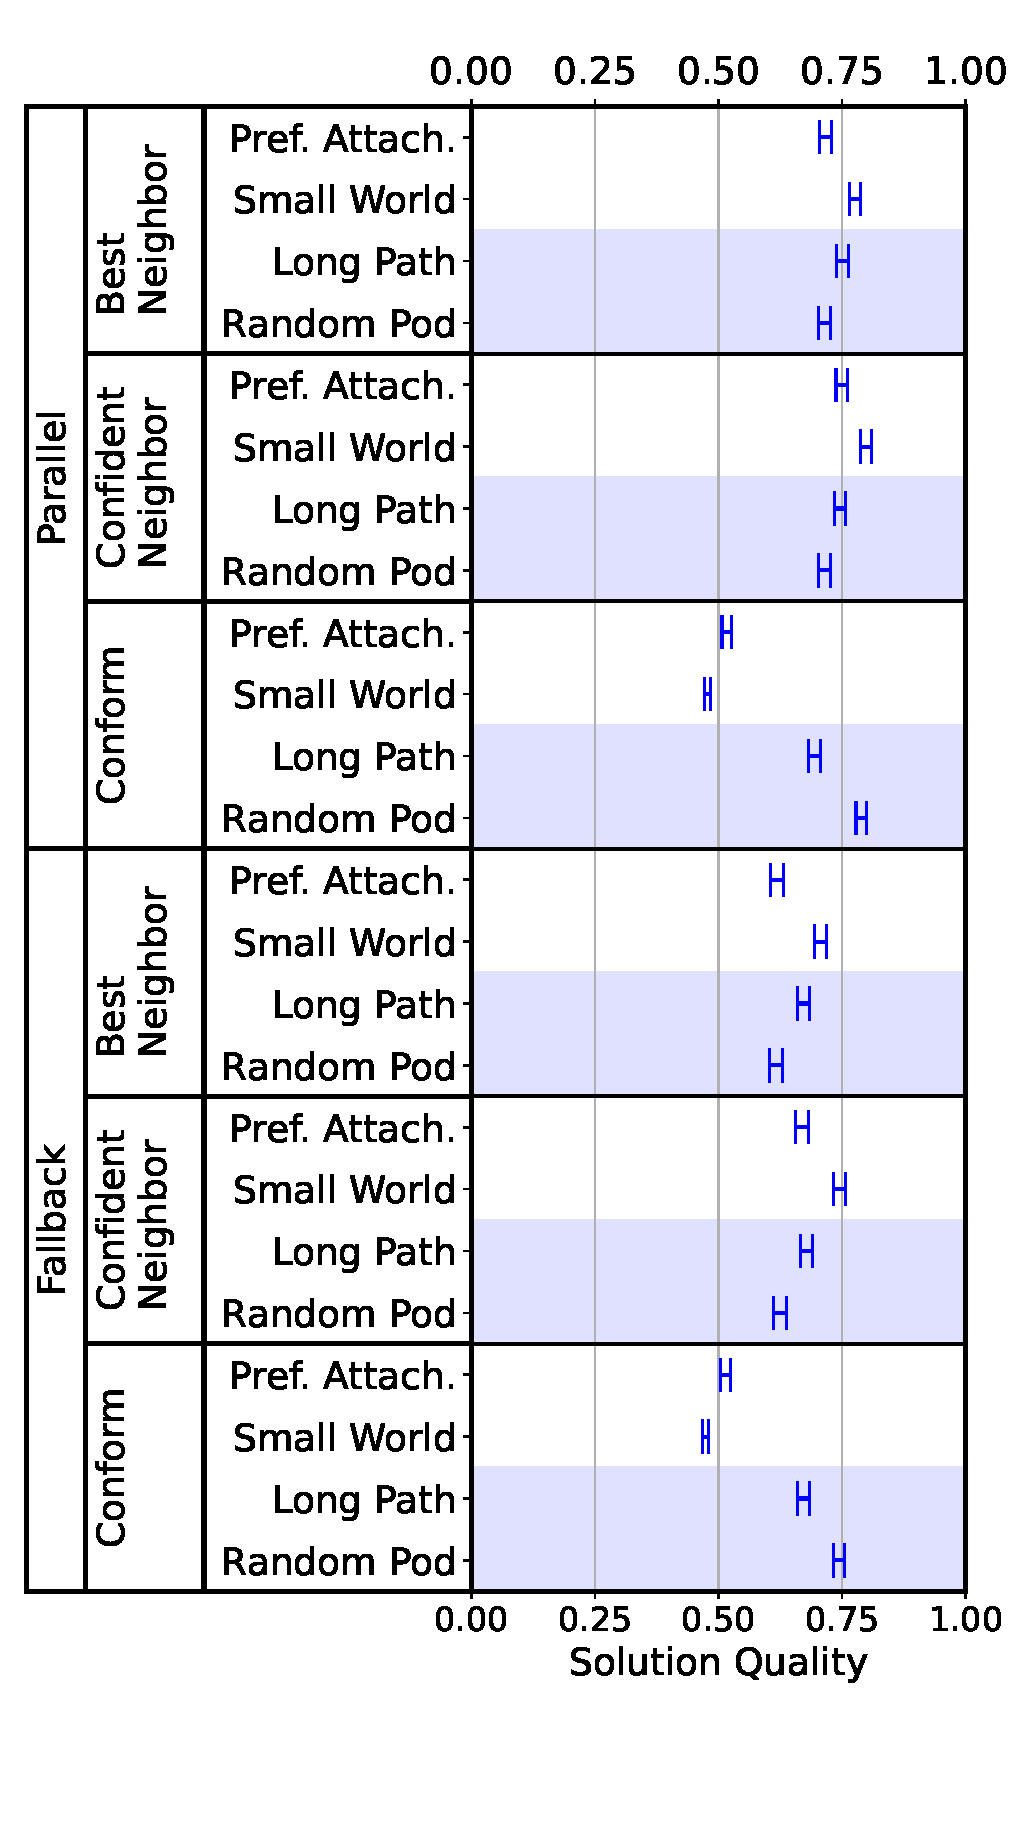
\includegraphics[width=3.33in]{fig/NetDelibABM/fig-perf-both.eps}
    \end{minipage}%
    \begin{minipage}{1.875in}
    \centering
    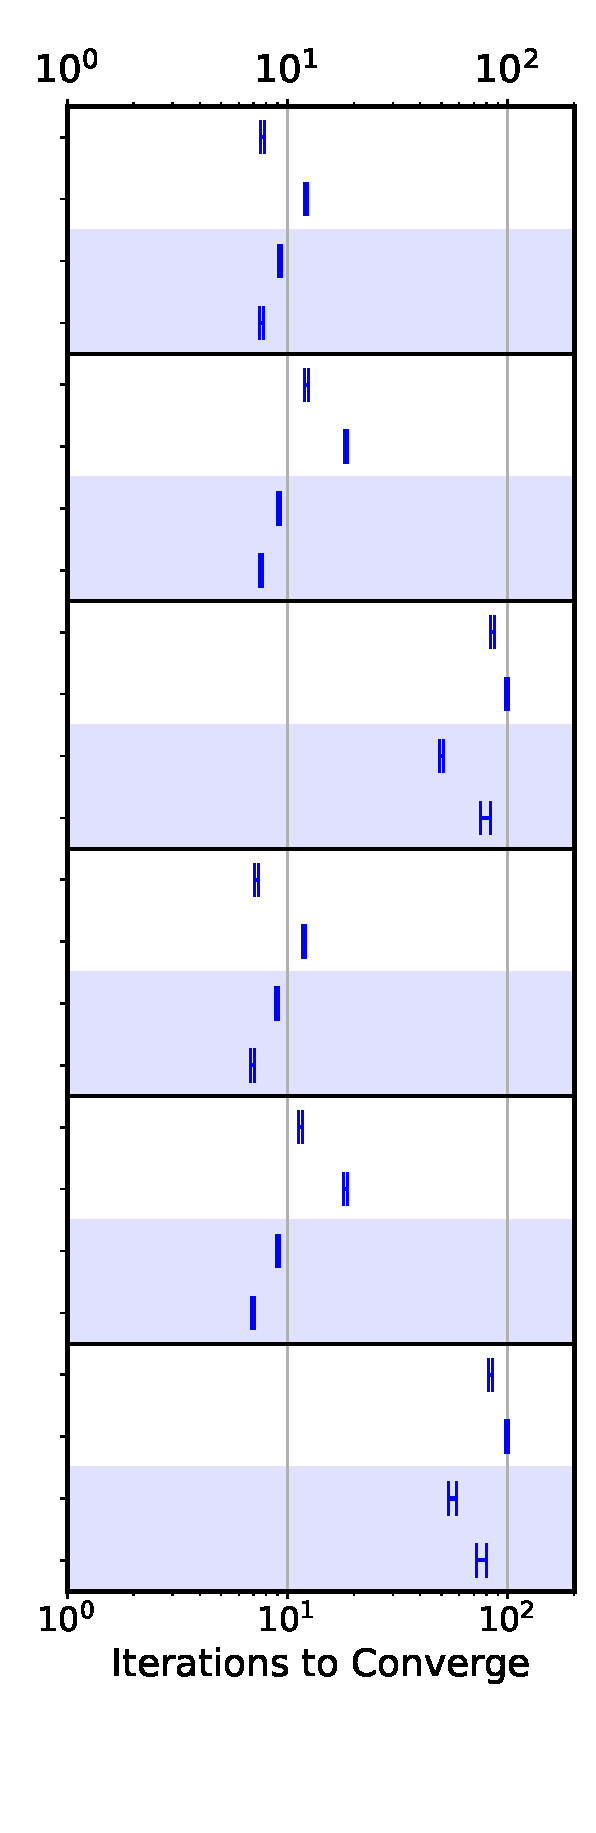
\includegraphics[width=1.875in]{fig/NetDelibABM/fig-converge-both.eps}
    \end{minipage}
\caption{
Solution quality and convergence time for agent-based simulations of different learning strategies. Error bars represent 95\% confidence interval. Results for network deliberation are shown shaded.
}
\end{figure*}

\begin{figure}
    \label{fig:results-frac-parallel}
    \centering
    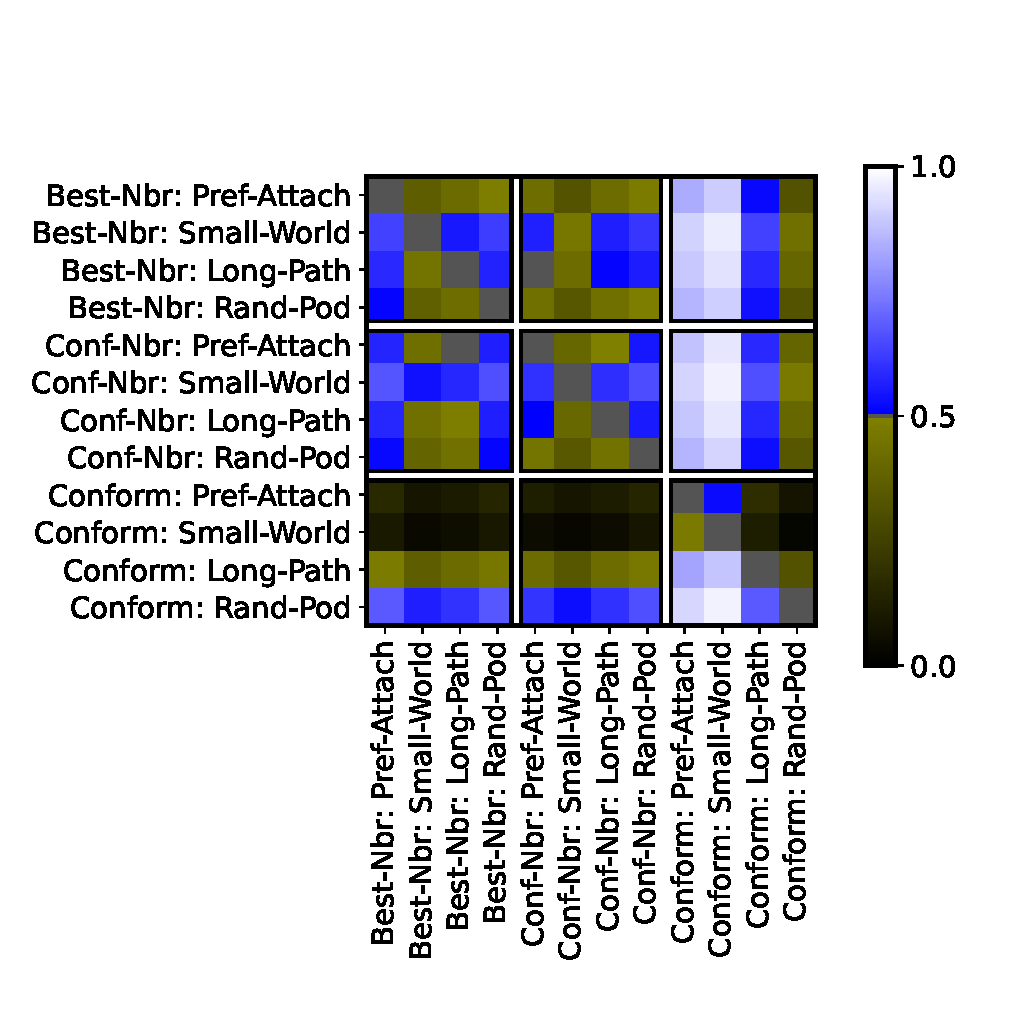
\includegraphics[width=3.33in]{fig/NetDelibABM/fig-result-frac-parallel.eps}
\caption{Fraction of simulations in which the row condition outperforms the column condition. Results are shown for parallel individual learning. In the case of a tie, weight is divided evenly.}
\end{figure}

\begin{figure}
    \label{fig:results-frac-fallback}
    \centering
%    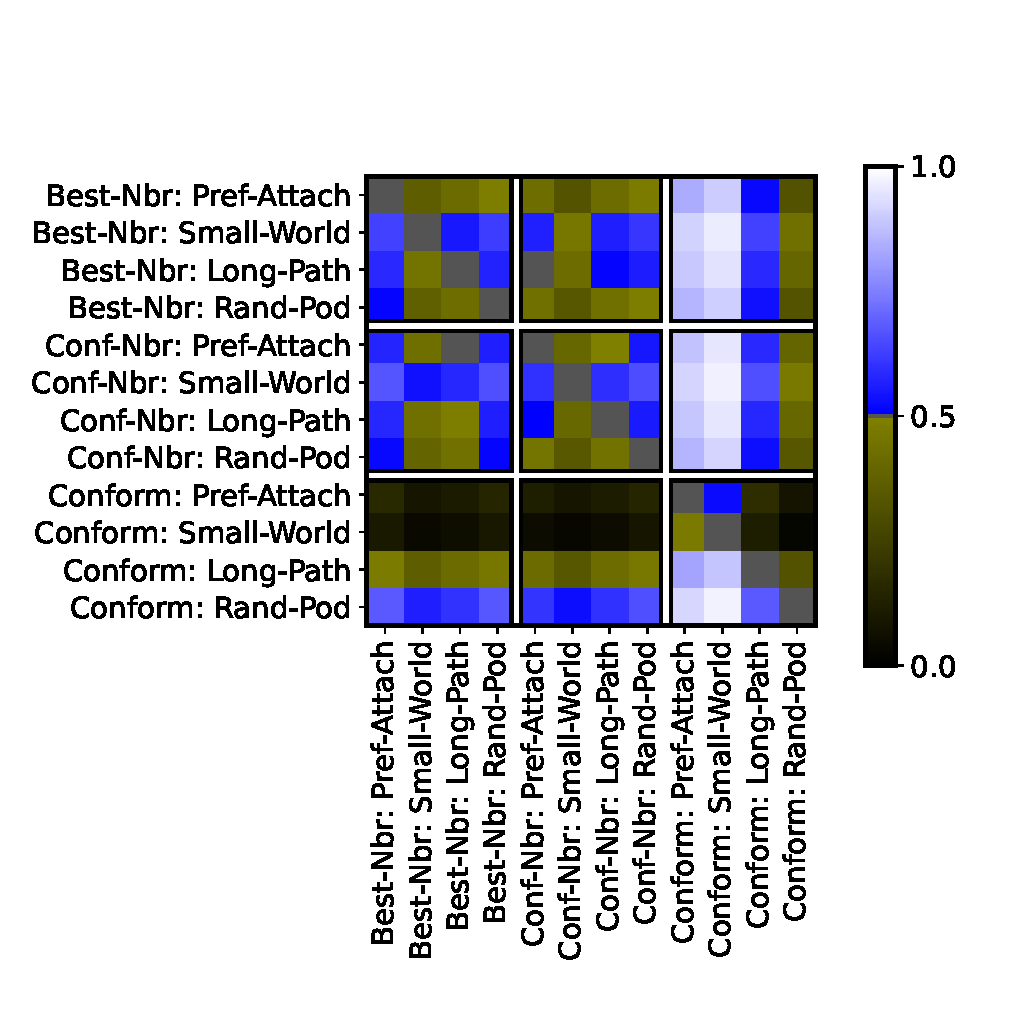
\includegraphics[width=3.33in]{fig/NetDelibABM/fig-result-frac-parallel.eps}
\caption{Fraction of simulations in which the row condition outperforms the column condition. Results are shown for fallback individual learning. In the case of a tie, weight is divided evenly.}
\end{figure}

\begin{figure}
    \label{fig:results-bn-parallel-dist}
    \centering
    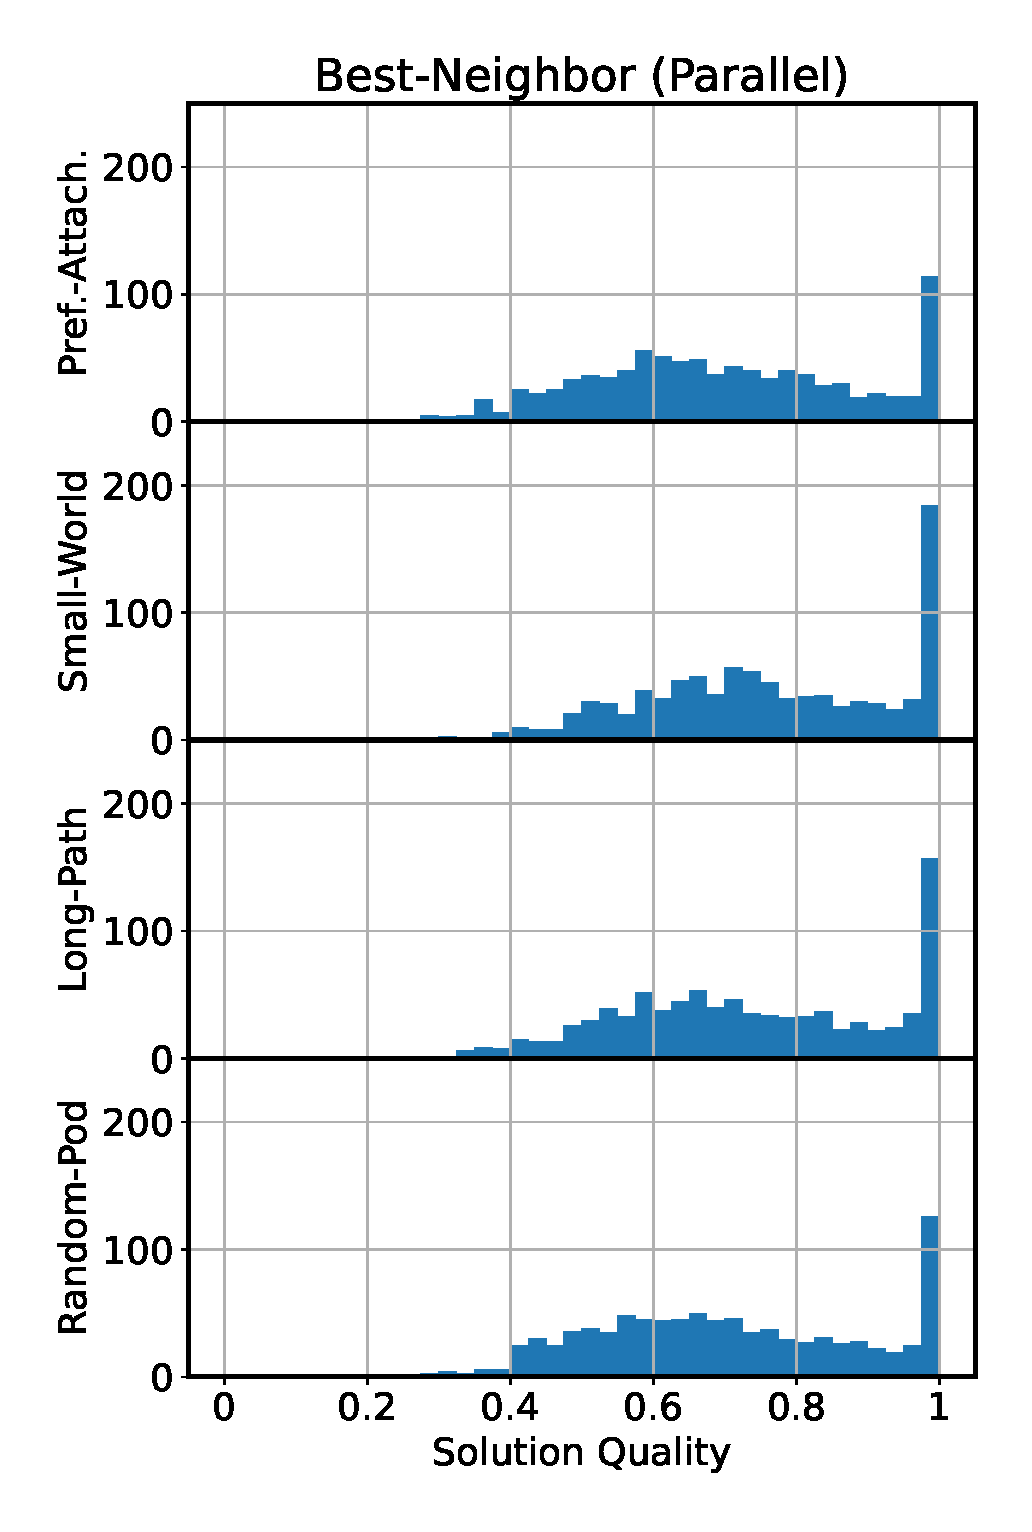
\includegraphics[width=3.33in]{fig/NetDelibABM/results-bn-parallel-dist.eps}
\caption{Solution quality distribution for best-neighbor strategy with parallel individual learning.}
\end{figure}
\begin{figure}
    \label{fig:results-cn-parallel-dist}
    \centering
    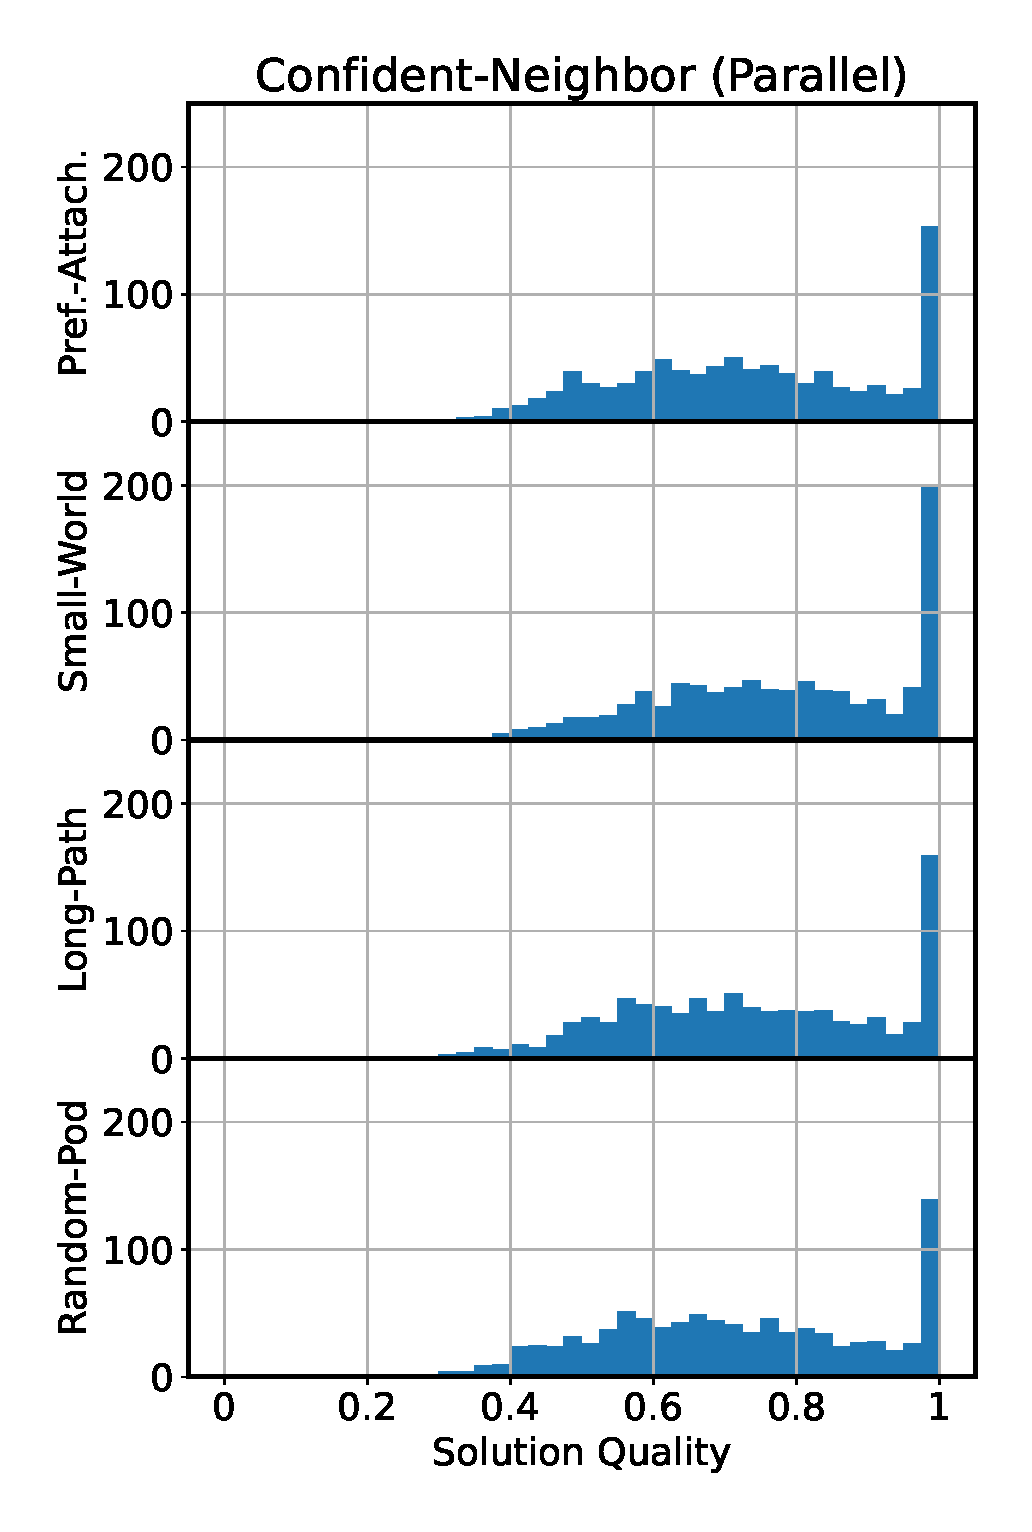
\includegraphics[width=3.33in]{fig/NetDelibABM/results-cn-parallel-dist.eps}
\caption{Solution quality distribution for confident-neighbor strategy with parallel individual learning.}
\end{figure}
\begin{figure}
    \label{fig:results-conf-parallel-dist}
    \centering
    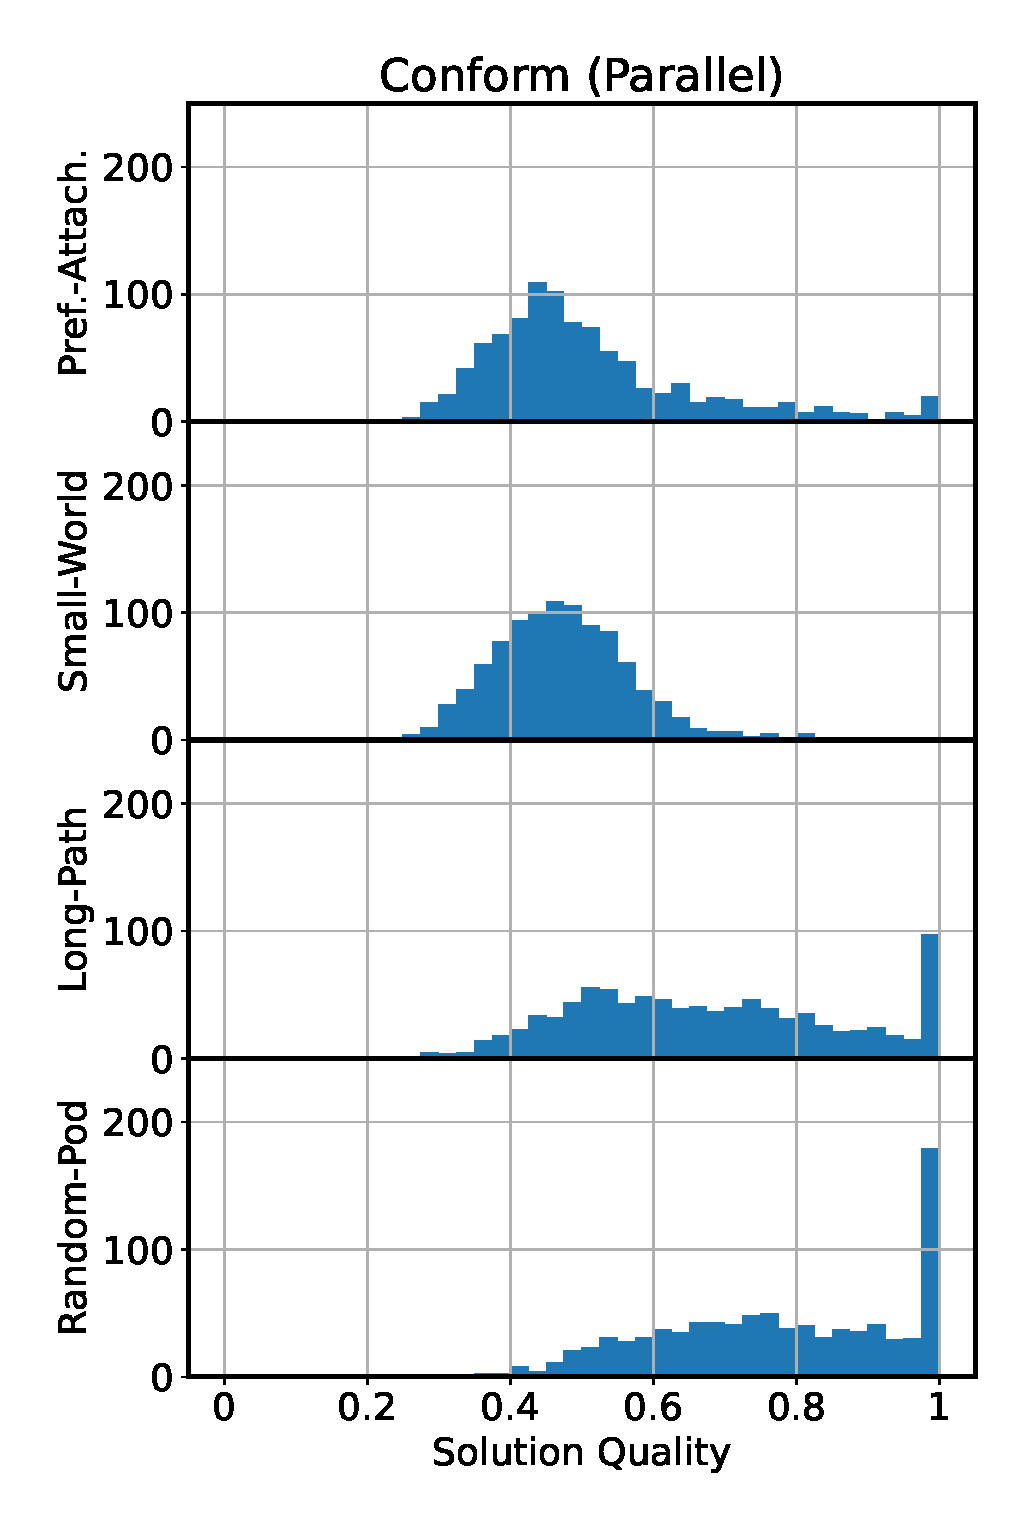
\includegraphics[width=3.33in]{fig/NetDelibABM/results-conf-parallel-dist.eps}
\caption{Solution quality distribution for the conform strategy with parallel individual learning.}
\end{figure}

\begin{figure}
    \label{fig:results-bn-fallback-dist}
    \centering
    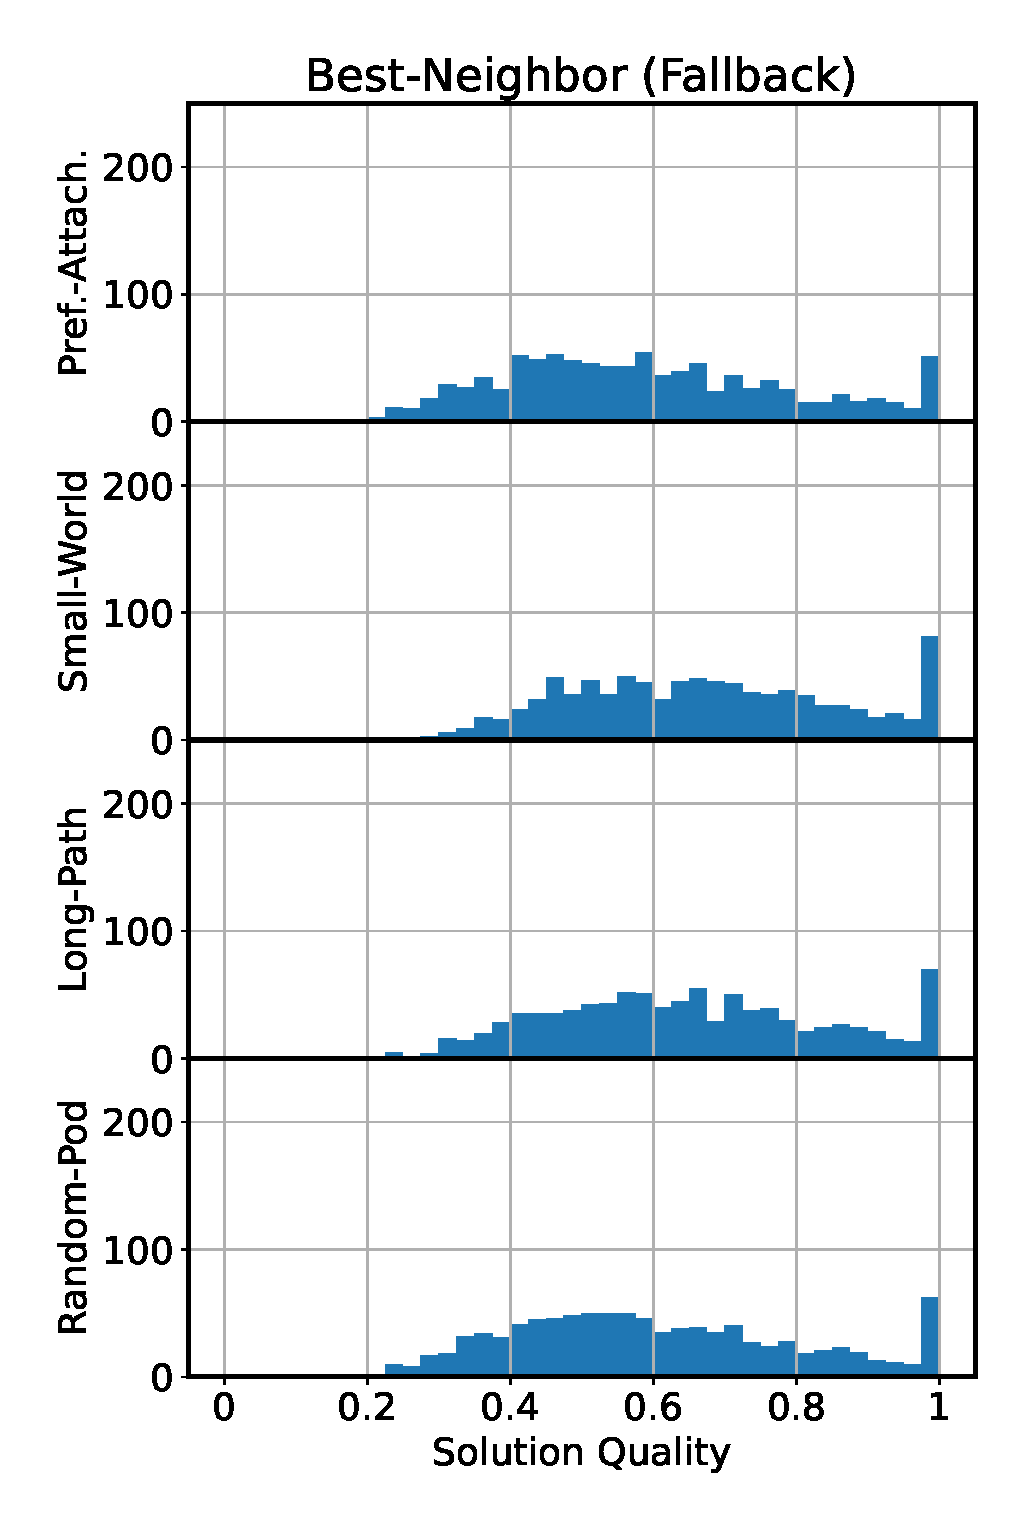
\includegraphics[width=3.33in]{fig/NetDelibABM/results-bn-fallback-dist.eps}
\caption{Solution quality distribution for best-neighbor strategy with fallback individual learning.}
\end{figure}
\begin{figure}
    \label{fig:results-cn-fallback-dist}
    \centering
    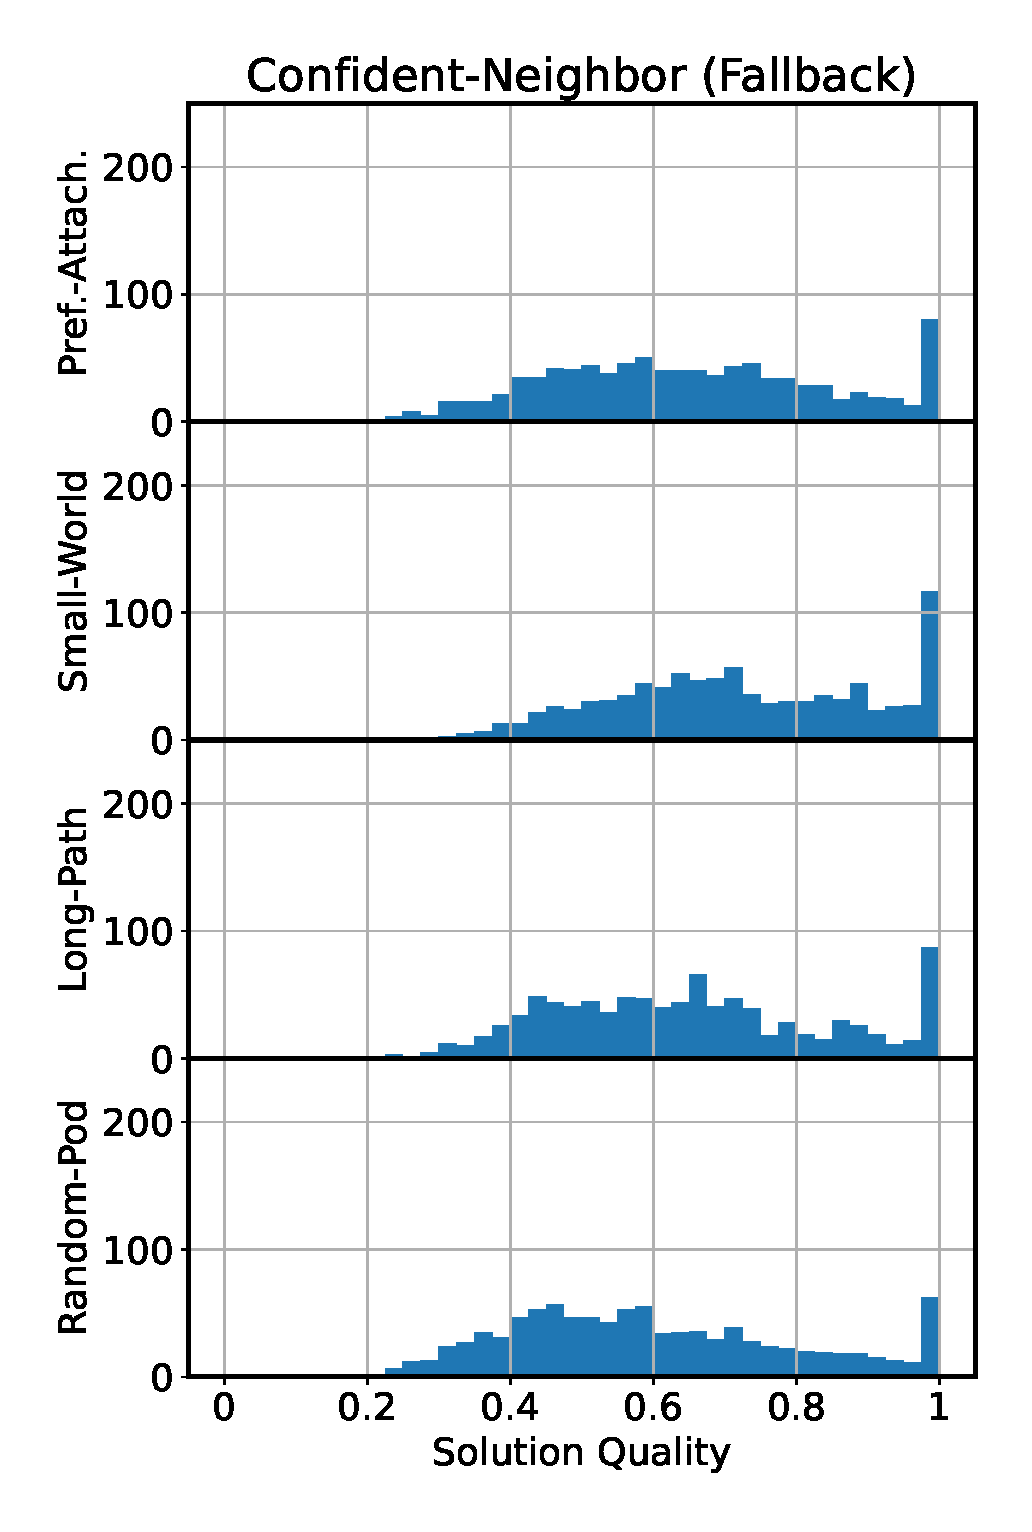
\includegraphics[width=3.33in]{fig/NetDelibABM/results-cn-fallback-dist.eps}
\caption{Solution quality distribution for confident-neighbor strategy with fallback individual learning.}
\end{figure}
\begin{figure}
    \label{fig:results-conf-fallback-dist}
    \centering
    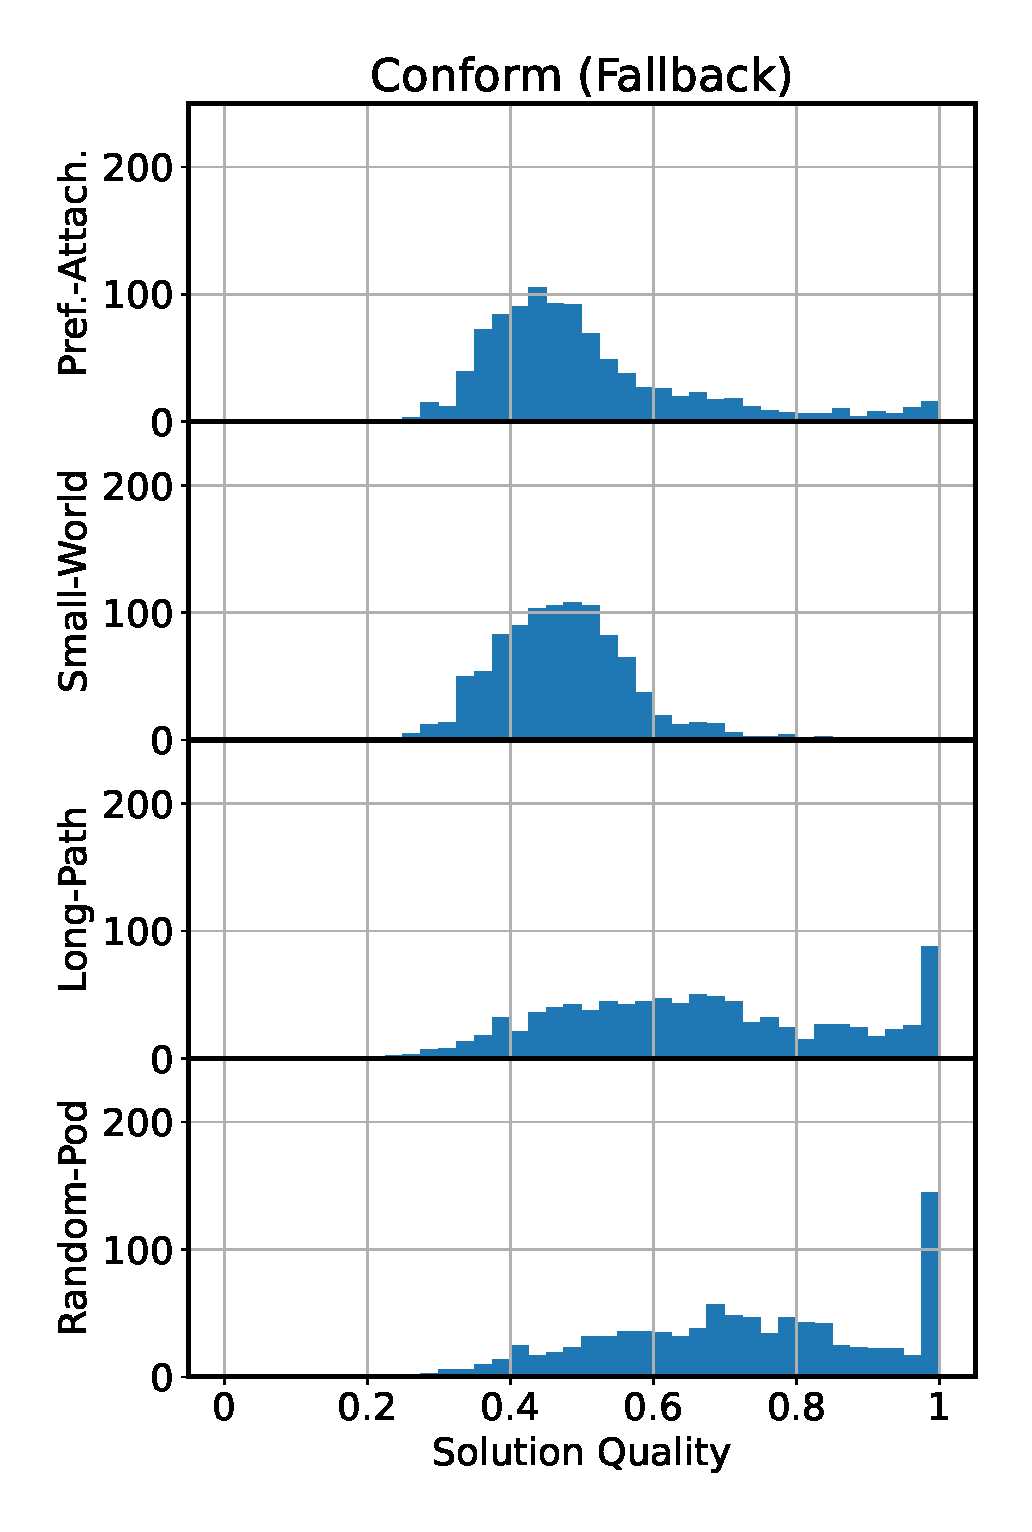
\includegraphics[width=3.33in]{fig/NetDelibABM/results-conf-fallback-dist.eps}
\caption{Solution quality distribution for the conform strategy with fallback individual learning.}
\end{figure}

\begin{table*}[]
    \label{tab:t-instrat-fallback}
    \centering
    \begin{tabular}{l|ll|ccc}
        Strategy & Net A & Net B & $\overline{B - A}$ & t & p* \\
        \hline
Best Neighbor&Pref. Attach.&Small World&-8.70e-02&-1.33e+01&1.27e-35\\
Best Neighbor&Pref. Attach.&Long Path&-5.98e-02&-8.62e+00&1.51e-15\\
Best Neighbor&Pref. Attach.&Random Pod&-1.15e-02&-1.83e+00&4.01e+00\\
Best Neighbor&Small World&Pref. Attach.&8.70e-02&1.33e+01&1.27e-35\\
Best Neighbor&Small World&Long Path&2.72e-02&4.53e+00&3.88e-04\\
Best Neighbor&Small World&Random Pod&7.55e-02&1.18e+01&1.66e-28\\
Best Neighbor&Long Path&Pref. Attach.&5.98e-02&8.62e+00&1.51e-15\\
Best Neighbor&Long Path&Small World&-2.72e-02&-4.53e+00&3.88e-04\\
Best Neighbor&Long Path&Random Pod&4.83e-02&7.34e+00&2.69e-11\\
Best Neighbor&Random Pod&Pref. Attach.&1.15e-02&1.83e+00&4.01e+00\\
Best Neighbor&Random Pod&Small World&-7.55e-02&-1.18e+01&1.66e-28\\
Best Neighbor&Random Pod&Long Path&-4.83e-02&-7.34e+00&2.69e-11\\
\hline
Confident Neighbor&Pref. Attach.&Small World&-7.52e-02&-1.13e+01&2.94e-26\\
Confident Neighbor&Pref. Attach.&Long Path&2.39e-03&3.64e-01&4.30e+01\\
Confident Neighbor&Pref. Attach.&Random Pod&5.80e-02&8.88e+00&1.86e-16\\
Confident Neighbor&Small World&Pref. Attach.&7.52e-02&1.13e+01&2.94e-26\\
Confident Neighbor&Small World&Long Path&7.76e-02&1.21e+01&1.08e-29\\
Confident Neighbor&Small World&Random Pod&1.33e-01&1.92e+01&1.36e-68\\
Confident Neighbor&Long Path&Pref. Attach.&-2.39e-03&-3.64e-01&4.30e+01\\
Confident Neighbor&Long Path&Small World&-7.76e-02&-1.21e+01&1.08e-29\\
Confident Neighbor&Long Path&Random Pod&5.56e-02&8.50e+00&4.00e-15\\
Confident Neighbor&Random Pod&Pref. Attach.&-5.80e-02&-8.88e+00&1.86e-16\\
Confident Neighbor&Random Pod&Small World&-1.33e-01&-1.92e+01&1.36e-68\\
Confident Neighbor&Random Pod&Long Path&-5.56e-02&-8.50e+00&4.00e-15\\
\hline
Conform&Pref. Attach.&Small World&3.60e-02&6.78e+00&1.24e-09\\
Conform&Pref. Attach.&Long Path&-1.63e-01&-2.22e+01&2.25e-87\\
Conform&Pref. Attach.&Random Pod&-2.28e-01&-3.19e+01&9.08e-153\\
Conform&Small World&Pref. Attach.&-3.60e-02&-6.78e+00&1.24e-09\\
Conform&Small World&Long Path&-1.99e-01&-3.17e+01&1.59e-151\\
Conform&Small World&Random Pod&-2.64e-01&-4.43e+01&2.20e-236\\
Conform&Long Path&Pref. Attach.&1.63e-01&2.22e+01&2.25e-87\\
Conform&Long Path&Small World&1.99e-01&3.17e+01&1.59e-151\\
Conform&Long Path&Random Pod&-6.48e-02&-8.31e+00&1.79e-14\\
Conform&Random Pod&Pref. Attach.&2.28e-01&3.19e+01&9.08e-153\\
Conform&Random Pod&Small World&2.64e-01&4.43e+01&2.20e-236\\
Conform&Random Pod&Long Path&6.48e-02&8.31e+00&1.79e-14\\
\hline
    \end{tabular}
    \caption{Two-tailed paired t-values across networks, within strategies. Results are for fallback individual learning. For all rows, dof=999 and $p^*$ is the Bonferroni-corrected p-value with m=60.}
\end{table*}

\begin{table*}[]
    \label{tab:t-innet-fallback}
    \centering
    \begin{tabular}{l|ll|ccc}
        Network & Strategy A & Strategy B & $\overline{B - A}$ & t & p* \\
        \hline
Pref. Attach.&Best Neighbor&Confident Neighbor&-6.43e-02&-9.39e+00&2.33e-18\\
Pref. Attach.&Best Neighbor&Conform&8.96e-02&1.19e+01&6.83e-29\\
Pref. Attach.&Confident Neighbor&Best Neighbor&6.43e-02&9.39e+00&2.33e-18\\
Pref. Attach.&Confident Neighbor&Conform&1.54e-01&2.06e+01&7.57e-77\\
Pref. Attach.&Conform&Best Neighbor&-8.96e-02&-1.19e+01&6.83e-29\\
Pref. Attach.&Conform&Confident Neighbor&-1.54e-01&-2.06e+01&7.57e-77\\
\hline
Small World&Best Neighbor&Confident Neighbor&-5.26e-02&-8.39e+00&9.70e-15\\
Small World&Best Neighbor&Conform&2.13e-01&3.52e+01&4.46e-175\\
Small World&Confident Neighbor&Best Neighbor&5.26e-02&8.39e+00&9.70e-15\\
Small World&Confident Neighbor&Conform&2.65e-01&4.45e+01&1.24e-237\\
Small World&Conform&Best Neighbor&-2.13e-01&-3.52e+01&4.46e-175\\
Small World&Conform&Confident Neighbor&-2.65e-01&-4.45e+01&1.24e-237\\
\hline
Long Path&Best Neighbor&Confident Neighbor&-2.12e-03&-3.42e-01&4.39e+01\\
Long Path&Best Neighbor&Conform&-1.37e-02&-1.71e+00&5.20e+00\\
Long Path&Confident Neighbor&Best Neighbor&2.12e-03&3.42e-01&4.39e+01\\
Long Path&Confident Neighbor&Conform&-1.16e-02&-1.44e+00&8.96e+00\\
Long Path&Conform&Best Neighbor&1.37e-02&1.71e+00&5.20e+00\\
Long Path&Conform&Confident Neighbor&1.16e-02&1.44e+00&8.96e+00\\
\hline
Random Pod&Best Neighbor&Confident Neighbor&5.18e-03&8.40e-01&2.41e+01\\
Random Pod&Best Neighbor&Conform&-1.27e-01&-1.64e+01&1.07e-51\\
Random Pod&Confident Neighbor&Best Neighbor&-5.18e-03&-8.40e-01&2.41e+01\\
Random Pod&Confident Neighbor&Conform&-1.32e-01&-1.67e+01&1.39e-53\\
Random Pod&Conform&Best Neighbor&1.27e-01&1.64e+01&1.07e-51\\
Random Pod&Conform&Confident Neighbor&1.32e-01&1.67e+01&1.39e-53\\
\hline
    \end{tabular}
    \caption{Two-tailed paired t-values across strategies, within networks. Results are for fallback individual learning. For all rows, dof=999 and $p^*$ is the Bonferroni-corrected p-value with m=60.}
\end{table*}

\begin{table*}[]
    \label{tab:t-instrat-parallel}
    \centering
    \begin{tabular}{l|ll|ccc}
        Strategy & Net A & Net B & $\overline{B - A}$ & t & p* \\
    \hline
Best Neighbor&Pref. Attach.&Small World&-6.75e-02&-1.13e+01&2.48e-26\\
Best Neighbor&Pref. Attach.&Long Path&-4.24e-02&-6.78e+00&1.25e-09\\
Best Neighbor&Pref. Attach.&Random Pod&-8.14e-03&-1.32e+00&1.12e+01\\
Best Neighbor&Small World&Pref. Attach.&6.75e-02&1.13e+01&2.48e-26\\
Best Neighbor&Small World&Long Path&2.50e-02&4.25e+00&1.42e-03\\
Best Neighbor&Small World&Random Pod&5.93e-02&9.38e+00&2.54e-18\\
Best Neighbor&Long Path&Pref. Attach.&4.24e-02&6.78e+00&1.25e-09\\
Best Neighbor&Long Path&Small World&-2.50e-02&-4.25e+00&1.42e-03\\
Best Neighbor&Long Path&Random Pod&3.43e-02&5.36e+00&6.14e-06\\
Best Neighbor&Random Pod&Pref. Attach.&8.14e-03&1.32e+00&1.12e+01\\
Best Neighbor&Random Pod&Small World&-5.93e-02&-9.38e+00&2.54e-18\\
Best Neighbor&Random Pod&Long Path&-3.43e-02&-5.36e+00&6.14e-06\\
\hline
Confident Neighbor&Pref. Attach.&Small World&-4.49e-02&-7.20e+00&7.03e-11\\
Confident Neighbor&Pref. Attach.&Long Path&-5.03e-03&-7.65e-01&2.67e+01\\
Confident Neighbor&Pref. Attach.&Random Pod&2.61e-02&4.02e+00&3.74e-03\\
Confident Neighbor&Small World&Pref. Attach.&4.49e-02&7.20e+00&7.03e-11\\
Confident Neighbor&Small World&Long Path&3.99e-02&6.96e+00&3.80e-10\\
Confident Neighbor&Small World&Random Pod&7.10e-02&1.18e+01&1.98e-28\\
Confident Neighbor&Long Path&Pref. Attach.&5.03e-03&7.65e-01&2.67e+01\\
Confident Neighbor&Long Path&Small World&-3.99e-02&-6.96e+00&3.80e-10\\
Confident Neighbor&Long Path&Random Pod&3.11e-02&4.89e+00&7.03e-05\\
Confident Neighbor&Random Pod&Pref. Attach.&-2.61e-02&-4.02e+00&3.74e-03\\
Confident Neighbor&Random Pod&Small World&-7.10e-02&-1.18e+01&1.98e-28\\
Confident Neighbor&Random Pod&Long Path&-3.11e-02&-4.89e+00&7.03e-05\\
\hline
Conform&Pref. Attach.&Small World&3.67e-02&6.85e+00&7.73e-10\\
Conform&Pref. Attach.&Long Path&-1.73e-01&-2.40e+01&7.10e-99\\
Conform&Pref. Attach.&Random Pod&-2.77e-01&-4.08e+01&6.29e-213\\
Conform&Small World&Pref. Attach.&-3.67e-02&-6.85e+00&7.73e-10\\
Conform&Small World&Long Path&-2.09e-01&-3.46e+01&3.46e-171\\
Conform&Small World&Random Pod&-3.14e-01&-5.68e+01&1.63e-313\\
Conform&Long Path&Pref. Attach.&1.73e-01&2.40e+01&7.10e-99\\
Conform&Long Path&Small World&2.09e-01&3.46e+01&3.46e-171\\
Conform&Long Path&Random Pod&-1.04e-01&-1.43e+01&8.55e-41\\
Conform&Random Pod&Pref. Attach.&2.77e-01&4.08e+01&6.29e-213\\
Conform&Random Pod&Small World&3.14e-01&5.68e+01&1.63e-313\\
Conform&Random Pod&Long Path&1.04e-01&1.43e+01&8.55e-41\\
    \hline
    \end{tabular}
    \caption{Two-tailed paired t-values across networks, within strategies. Results are for parallel individual learning. For all rows, dof=999 and $p^*$ is the Bonferroni-corrected p-value with m=60.}
\end{table*}

\begin{table*}[]
    \label{tab:t-innet-parallel}
    \centering
    \begin{tabular}{l|ll|ccc}
        Network & Strategy A & Strategy B & $\overline{B - A}$ & t & p* \\
    \hline
Pref. Attach.&Best Neighbor&Confident Neighbor&-3.78e-02&-5.94e+00&2.39e-07\\
Pref. Attach.&Best Neighbor&Conform&2.00e-01&2.77e+01&3.28e-124\\
Pref. Attach.&Confident Neighbor&Best Neighbor&3.78e-02&5.94e+00&2.39e-07\\
Pref. Attach.&Confident Neighbor&Conform&2.38e-01&3.40e+01&1.67e-167\\
Pref. Attach.&Conform&Best Neighbor&-2.00e-01&-2.77e+01&3.28e-124\\
Pref. Attach.&Conform&Confident Neighbor&-2.38e-01&-3.40e+01&1.67e-167\\
\hline
Small World&Best Neighbor&Confident Neighbor&-1.52e-02&-2.74e+00&3.80e-01\\
Small World&Best Neighbor&Conform&3.05e-01&5.30e+01&1.25e-290\\
Small World&Confident Neighbor&Best Neighbor&1.52e-02&2.74e+00&3.80e-01\\
Small World&Confident Neighbor&Conform&3.20e-01&5.89e+01&0.00e+00\\
Small World&Conform&Best Neighbor&-3.05e-01&-5.30e+01&1.25e-290\\
Small World&Conform&Confident Neighbor&-3.20e-01&-5.89e+01&0.00e+00\\
\hline
Long Path&Best Neighbor&Confident Neighbor&-3.88e-04&-6.64e-02&5.68e+01\\
Long Path&Best Neighbor&Conform&7.02e-02&9.34e+00&3.64e-18\\
Long Path&Confident Neighbor&Best Neighbor&3.88e-04&6.64e-02&5.68e+01\\
Long Path&Confident Neighbor&Conform&7.06e-02&9.15e+00&1.83e-17\\
Long Path&Conform&Best Neighbor&-7.02e-02&-9.34e+00&3.64e-18\\
Long Path&Conform&Confident Neighbor&-7.06e-02&-9.15e+00&1.83e-17\\
\hline
Random Pod&Best Neighbor&Confident Neighbor&-3.59e-03&-5.46e-01&3.51e+01\\
Random Pod&Best Neighbor&Conform&-6.84e-02&-9.54e+00&6.11e-19\\
Random Pod&Confident Neighbor&Best Neighbor&3.59e-03&5.46e-01&3.51e+01\\
Random Pod&Confident Neighbor&Conform&-6.48e-02&-8.96e+00&9.43e-17\\
Random Pod&Conform&Best Neighbor&6.84e-02&9.54e+00&6.11e-19\\
Random Pod&Conform&Confident Neighbor&6.48e-02&8.96e+00&9.43e-17\\
    \hline
    \end{tabular}
    \caption{Two-tailed paired t-values across strategies, within networks. Results are for parallel individual learning. For all rows, dof=999 and $p^*$ is the Bonferroni-corrected p-value with m=60.}
\end{table*}


\subsection{Network vs. Conventional Deliberation}
We are particularly interested in comparing the performance of network deliberation to that of conventional single-group deliberation. When the conform strategy is used, we find that both of the network deliberation conditions yield better performance than conventional networks (Figure \ref{fig:results-conform-diff}). Analysis of the solution quality distributions (Figure \ref{fig:results-conform-dist}) shows two distinct effects. First, network deliberation frequently finds maximal solutions while conventional deliberation does not. Second, even when non-maximal solutions are found, network deliberation finds higher-quality solutions. This benefit is robust across both parallel and fallback individual learning. The effect size is dramatic. Conventional networks combined with the conform strategy show the lowest performance of all conditions, while random pod network deliberation combined with the conform strategy shows higher performance than nearly all other conditions. The exception being small world network combined with the best/confident-neighbor strategy, which shows equal performance within our statistical resolution. 
Often, increased performance comes at the expense of speed as more time is devoted to exploring novel solutions. However, we find that network deliberation improves both performance and speed when the conform strategy is used, suggesting that interlocking network structure can enable more efficient exploration.

\begin{figure}
    \label{fig:results-conform-diff}
    \centering
    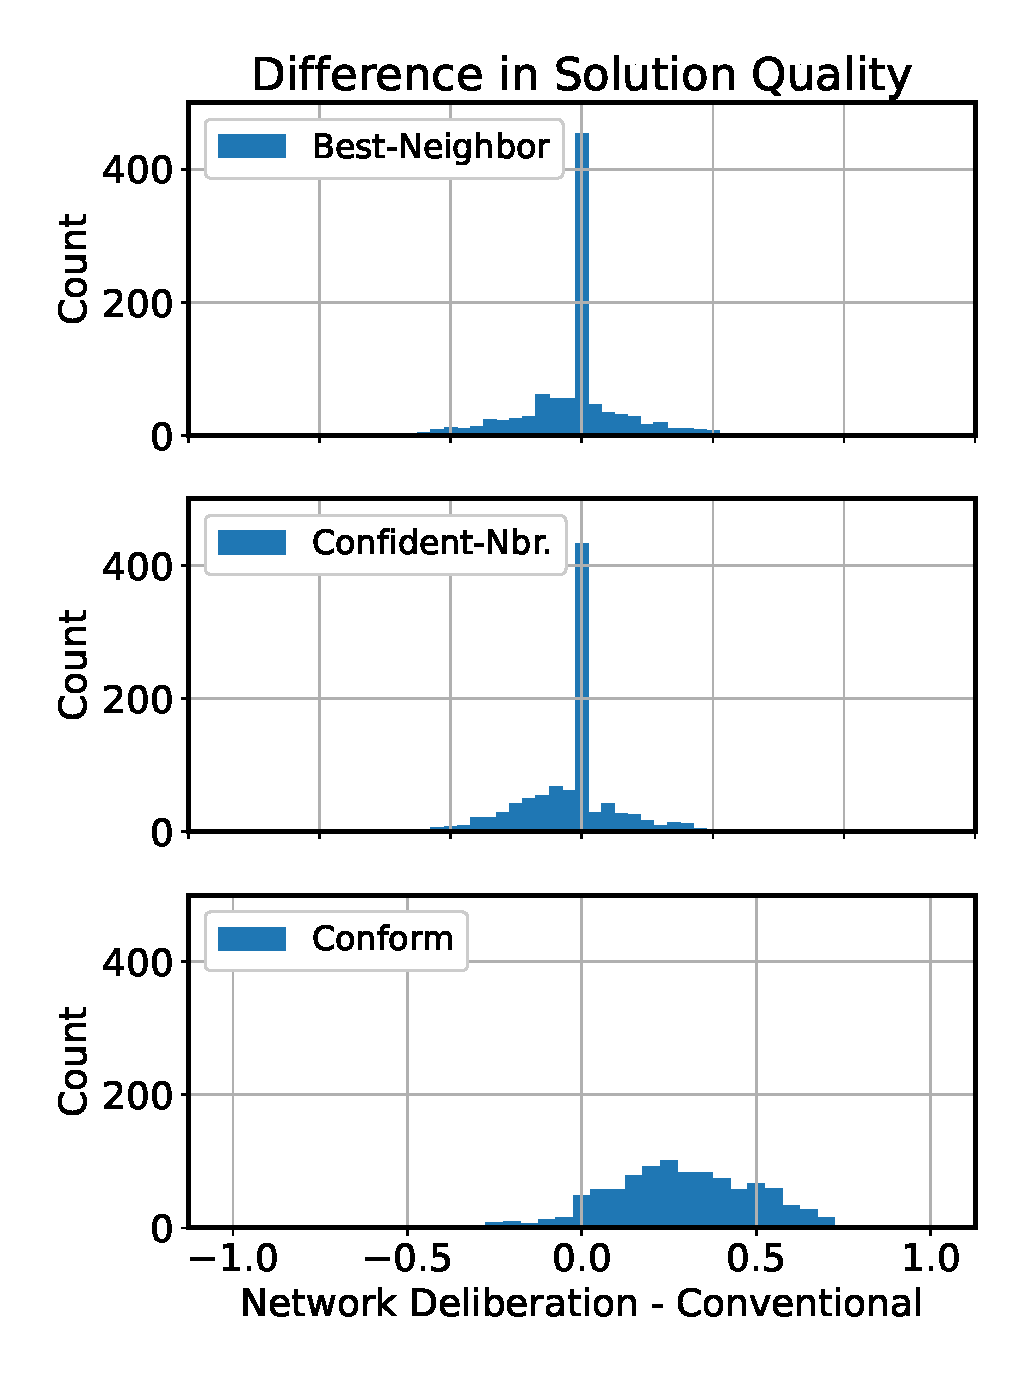
\includegraphics[width=3.33in]{fig/NetDelibABM/fig-results-netdelib-diff.eps}
\caption{Difference in solution quality between network deliberation and conventional deliberation. Plots for Best/Confident-Neighbor show results for long-path and small-world networks, while the plot for conform shows results for random-pod and preferential-attachment networks. Results are shown for parallel individual learning.}
\end{figure}

\begin{figure}
    \label{fig:results-conform-dist}
    \centering
    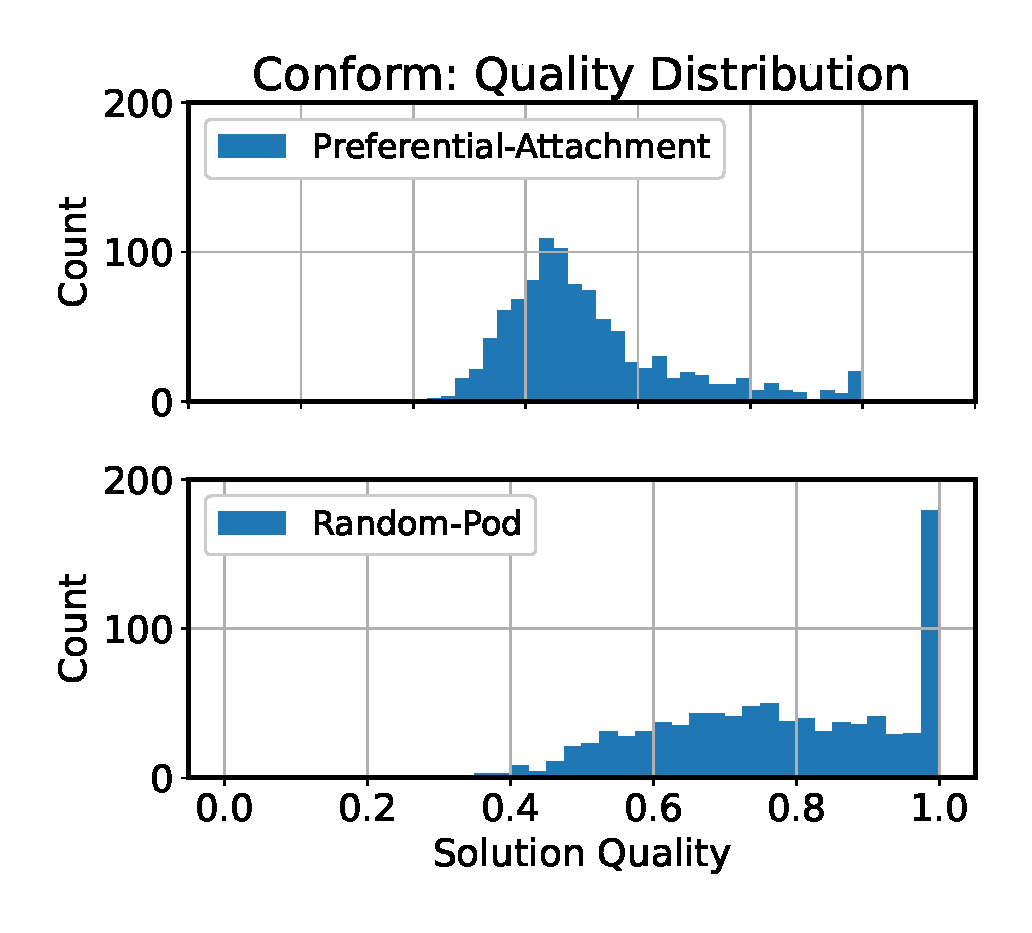
\includegraphics[width=3.33in]{fig/NetDelibABM/fig-results-conform-dist.eps}
\caption{Distributions of solution quality for social learning on a preferential-attachment network and random-pod network deliberation. Results are shown for parallel individual learning.}
\end{figure}

The conform strategy models contexts in which individuals rely heavily on social influence. Such contexts can arise from pro-conformity social norms, high levels of trust, social loafing, and limited information. As a form of rational ignorance, conformist behavior can conserve individual resources, but poses the risk of forming information cascades and propagating misinformation and inferior or harmful innovations \cite{banerjee_simple_1992}. Our simulations show that network deliberation can greatly improve the outcome of deliberation in the presence of strong social influence. This insight suggests one possible mechanism behind the success of mass deliberative projects, as well as the potential for network-based interventions in mass deliberation.

\subsection{Structural Efficiency}

The speed at which information can move through a communication network, i.e., it's structural efficiency, has been found to influence the success of collective problem-solving. We might expect the same to be true in network deliberation. In network deliberation, network structure is created through group membership. We compare the results of two group assignment methods: a random pod assignment yielding an efficient network, and a long-path method yielding a less efficient network (Figure \ref{fig:results-netdelib-efficiency}). We find that for greedy strategies (best-neighbor and confident-neighbor), the inefficient network yields the better results. The results are opposite for the conform strategy, with the efficient network yielding better results. These results are consistent with those observed for conventional single-group networks \cite{barkoczi_social_2016}, but to the best of our knowledge, they had not been explored for interlocking network like the ones we use to model network deliberation.

\begin{figure}
    \label{fig:results-netdelib-efficiency}
    \centering
    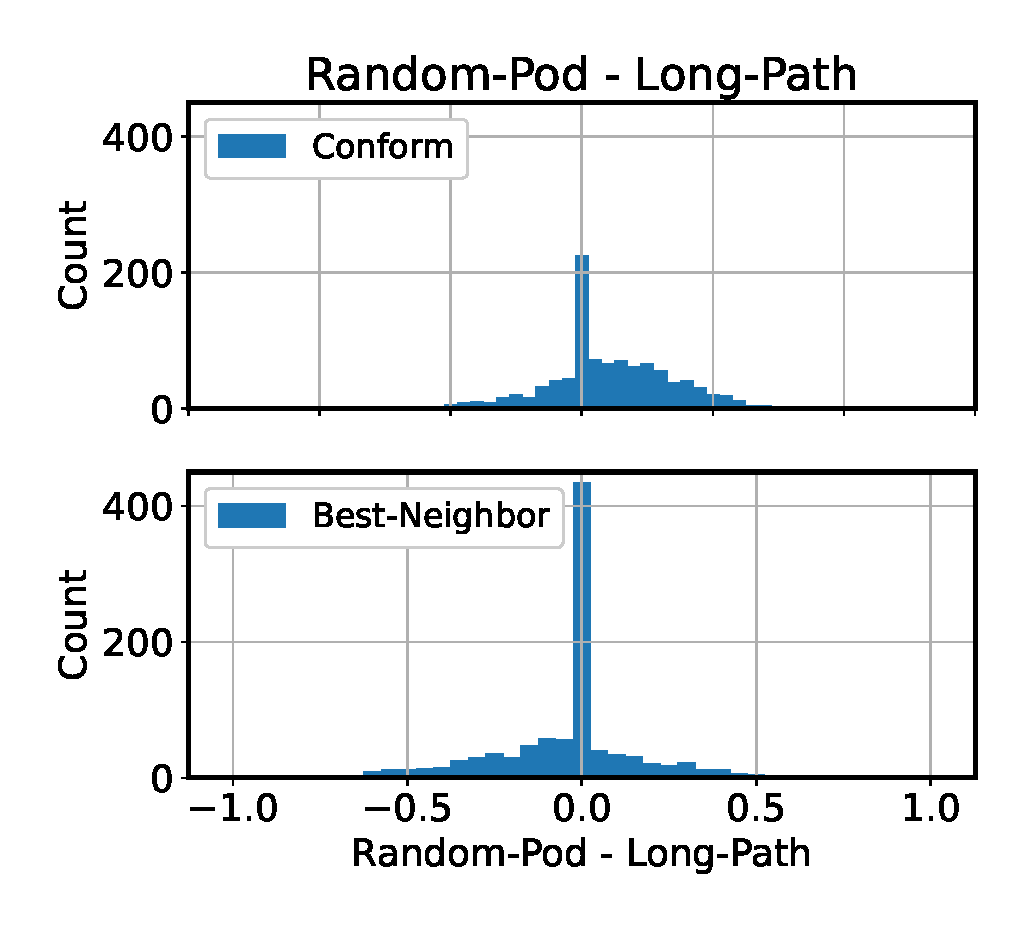
\includegraphics[width=3.33in]{fig/NetDelibABM/fig-results-netdelib-efficiency.eps}
\caption{Difference in solution quality between random-pod (efficient) and long-path (inefficient) network. Results are shown for parallel individual learning.}
\end{figure}

The role of structural efficiency in collective tasks can be partially attributed to diversity \cite{lazer_network_2007, hong_groups_2004}. Greedy strategies such as best/confident-neighbor result in agents adopting the highest quality solution they have seen so far and discarding all others. Such strategies quickly reduce the number of solutions present in the population, quickly identifying a local maximum at the cost of diversity. As a result, agents duplicate efforts during individual learning, exploring mutations of the same solution. Inefficient networks can mitigate this effect by slowing the spread of high-quality solutions and allowing time for the exploration of new and potentially better solutions. Our results show exactly this, with long-path pod assignment improving the performance of greedy algorithms. The improved performance of the conform strategy in random pod assignment can be attributed to the converse of the above. When social influence is strong, efficient networks can interrupt information cascades by introducing new information from far across the network.
Our results are thus generally consistent with existing theory on structural efficiency and collective problem-solving.
However, we note an interesting deviation: under the conform strategy, long-path network deliberation out-performs the two conventional networks, both of which are more efficient.

\subsection{Confident-Neighbor Strategy}

In general, the best-neighbor strategy requires strong assumptions about agents' ability to evaluate solutions. In the special case of network deliberation, the assumptions can be weakened by applying a variant of the strategy, which has not been previously studied. The variant, which we call {\em confident-neighbor}, is equivalent to best-neighbor for network deliberation, but not in general. Confident-neighbor thus provides a comparison between network deliberation and conventional single-group deliberation under weaker informational assumptions than best-neighbor. Surprisingly, the weaker assumptions of confident-neighbor lead to higher performance on the preferential attachment network, and similar performance on the-small world network (within our statistical resolution). Figure \ref{fig:results-confident} shows histograms of the quality difference between confident-neighbor and best-neighbor for both conventional networks. In the majority of cases, both strategies find comparable solutions. However, we find that when these strategies do find different solutions, those found by confident-neighbor are more often better, at least for the preferential-attachment network.

\begin{figure}
    \label{fig:results-confident}
    \centering
    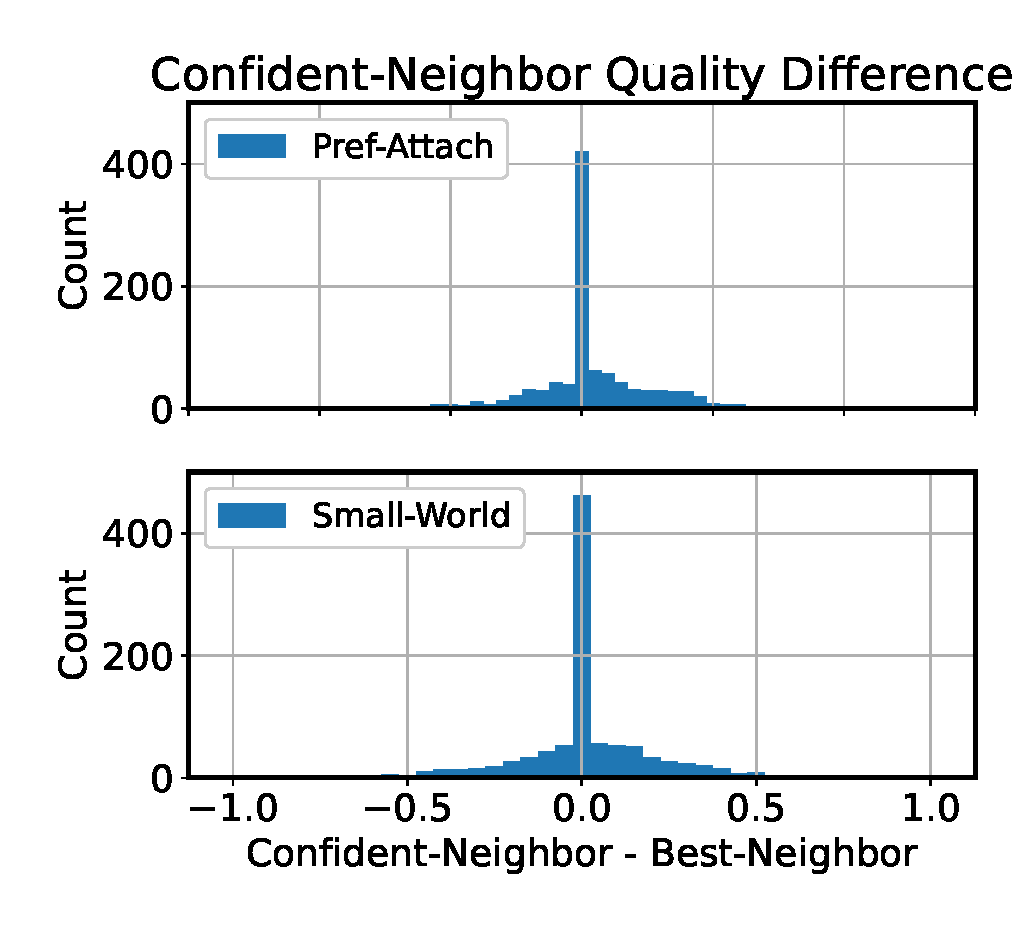
\includegraphics[width=3.33in]{fig/NetDelibABM/fig-results-confident.eps}
\caption{Histograms of the difference in solution quality between confident-neighbor and best-neighbor for both conventional networks.
Results are shown for parallel individual learning.}
\end{figure}

As with conform, the confident-neighbor strategy can be used when available information is insufficient to use best-neighbor. Unlike conform, confident-neighbor models weak social influence. The improved performance of confident-neighbor over best-neighbor, despite using less information, can be attributed at least in part to diversity and exploration. Confident neighbor takes significantly longer to converge, suggesting it maintains a diversity of solutions and allows more time to explore new solutions. Our results suggest several interventions with the potential to improve conventional single-group deliberation. In the presence of weak social influence, reducing the amount of information available can counter-intuitively increase performance. Conversely, when information is already limited, performance might be increased by weakening social influence. However, while confident-neighbor can increase the success of conventional deliberation, it performs comparably to network deliberation using the conform strategy, suggesting that when social influence is strong, network deliberation remains preferable.

\section{Discussion}

We have proposed and evaluated a model of mass deliberation based on the observed interlocking network structure of successful mass-deliberative projects.
Our central finding suggests that network deliberation can improve deliberative output in the presence of strong social influence (i.e., the conform strategy).
Individuals rely on social influence for a number of reasons.
Strong social influence can stem from social factors such as trust or social loafing.
Alternatively, social influence can be used to supplement individual skill when it is insufficient for a given task.
We see that a variety of contexts can lead to reliance on social influence.
Empirical evidence suggests the presence of strong social influence in real-world collaborations such as Wikipedia \cite{platt_network_2018} and in lab studies of human collaboration \cite{mason_collaborative_2012, barkoczi_social_2016}.
In the case of weak social influence (i.e., the  best-neighbor and confident-neighbor strategies), we do not observe a significant difference in output quality between network deliberation and conventional single-group deliberation. In all cases, network deliberation performs better than single-group deliberation or comparatively well. 
Our results suggest that network deliberation is both a contributing mechanism to the success of mass-deliberative projects as well as a useful tool for the design of large-scale sociotechnical systems and interventions for existing systems.

How does network deliberation improve collaborative output? In part, the high performance of random-pod network deliberation can be attributed to the high structural efficiency of the resulting network. However, structural efficiency cannot be the complete mechanism. Long-path network deliberation is extremely inefficient, but still outperforms conventional networks in the presence of strong social influence. The additional mechanisms at play remain an open question.

In order to distinguish between the effects of social influence and individual ability, we have introduced the confident-neighbor strategy, which (unlike best-neighbor) assumes the same agent capabilities as the conform strategy (in a critical learning setting).
While not central to our study of network deliberation, our findings regarding the 
confident-neighbor strategy have important implications for the study of social learning in general. 
Our findings show that just as reducing network efficiency can improve solution quality by raising diversity, reducing the available information can improve the performance of greedy learning strategies. Our investigation of confident-neighbor stems from a careful formal analysis of the information required by each strategy. The surprisingly high performance of confident-neighbor shows the importance of isolating social influence from agent ability.

Our work is limited by a number of assumptions, which require further investigation to achieve greater generalizability. We assume a static objective function, while real-world objectives can change with changing external conditions as well as changing individual preferences. We also assume a homogeneous strategy across all agents, which raises questions of how different strategies interact within the same collaboration. We have also assumed that agents are truthful and do not form coalitions outside of the existing network, both assumptions which can be violated in real-world settings.
We have also assumed that agents have access to the full solution string, and that agents incorporate all bits of the string into their quality estimates. Extremely complex real-world tasks might be better-modeled by a collection of sub-tasks, with agents having access to only a subset of the solution string.
Finally, we have limited our study to learning strategies that explore new solutions solely through small mutations of existing solutions. Other potential strategies might generate entirely new solutions, for example, by combining parts of multiple previous solutions. Such generative strategies would add the ability to explore a wider range of solutions. While our work extends the understanding of social learning and collaboration, many questions still remain open for exploration.

Effective mass deliberation is key to realizing the democratizing power of the internet. Our findings suggest that the presence of small and interlocking pods can contribute to the success of mass deliberation, particularly when the topic is complex and social influence is strong. These findings have implications for a range of deliberative contexts: participatory government and budgeting, worker-owned cooperatives, grassroots social movements, and the governance of decentralized systems (e.g., cryptocurrency). By enabling better deliberation at larger scales, we hope this work will contribute to democratizing the governance of large sociotechnical systems, and empowering the individuals impacted by those systems.



\chapter{Experimental evaluation of Network Deliberaiton}
\label{chap:experiment}
\section{Introduction}



\section{Experimental Design}

This section describes the experimental design of the proposed field experiment.
In this experiment, participants will use a pseudonymous online platform
to deliberate on a policy issue.
The deliberation will take place asynchronously, over a period of several days.
At several times throughout the deliberation,
participants will complete a ranked-choice poll regarding the policy issue,
allowing the evolution of their preferences to be tracked over the course of the
experiment.
Depending on opportunity and necessity, multiple waves of deliberation may
be conducted, each with a distinct policy issue and set of participants.


\subsection{Deliberative Topic}
The policy issue chosen as the topic of deliberation is a crucial component
of the experiment.
The topic will be chosen carefully according to several criteria.
The chosen policy issue must be:
\begin{itemize}
\item Relevant to the experimental population;
\item Amenable to participants changing their preferences based on new information or reasoning;
\item Amenable to a predefined list of proposed solutions;
\item Sufficiently complex to have three or more proposed solutions;
\item Timely, but unlikely to be influenced by current events during the deliberation.
\end{itemize}
Examples of policy issues meeting these criteria include:
\begin{itemize}
\item ``Where should the use of electric scooters be permitted?''
\item ``Given the COVID-19 pandemic, how should schools in the US reopen in Fall 2021?''
\end{itemize}


\subsection{Participant Recruitment and Incentives}
Participants will be recruited using several methods.
Participants will be recruited individually through posts on web forums
relevant to the policy question (e.g., reddit, facebook groups)
and to relevant email lists.
Participant pools will also be utilized,
including lists of previous participants
who have expressed interest in future studies
and the UMSI Online Recruitment System for Economic Experiments.
Individual participants will also be recruited using promoted posts and
advertisements on Twitter, Facebook, etc.
Separately, participants may also be recruited through partnership with
community groups who wish to try network deliberation as part of an organizational
decision-making strategy.
The number of such collaborations will depend on the number of interested
partner organizations that have decisions amenable to network deliberation
over the course of the experiment.

In order to incentivize participation and to compensate participants fairly
for their time,
participants who complete the deliberation and pre/post-experiment surveys
will be compensated financially.
Participants will be paid a predetermined fixed amount in order to
minimize the effect of the compensation on their deliberative behavior and
expressed preferences.


\subsection{Experimental Protocol}

Before the deliberation period begins,
participants will complete a short demographic survey.
This survey will enable the identification of sample bias in age, gender, race,
and other demographic factors.

Participants will be randomly assigned to one of three treatment/control groups
at time of enrollment:
\begin{description}
\item[Control]{
The control group will engage in conventional single large group deliberation.
Posts and comments made by participants in the control group will be visible
to all others in the control group for the entire duration of the deliberation.}
\item[Network Deliberation (Efficient)]{
Participants in this treatment group will be divided into small
(4--5 participant) pods.
Posts and comments made by participants in this treatment group will only be
visible to others in their current pod.
All participants will be assigned to a new pod at the beginning of each round
of deliberation using the random-pod assignment method,
producing a structurally efficient communication network.}
\item[Network Deliberation (Inefficient)]{
Participants in this treatment group will be divided into small
(4--5 participant) pods.
Posts and comments made by participants in this treatment group will only be
visible to others in their current pod.
All participants will be assigned to a new pod at the beginning of each round
of deliberation using the long-path assignment method,
producing a structurally inefficient communication network.}
\end{description}

The deliberation period will be divided into a predetermined number of {\em rounds},
each lasting a fixed length of time.
Present plans are to divide the deliberation period into three stages of two days
each.
However, these numbers may be adjusted to ensure time timeline of the
deliberation is consistent with any constraints imposed by specific policy issues.
Before and after each stage, participants will be asked to rank the proposed
solutions to the policy question according to their individual preference.
During each round, participants will be shown a discussion prompt and will be
able to post a response to that prompt.
Example prompts are shown in Table \ref{tab:prompts}.
Participants will be able to view and comment on the posts of other participants
assigned to the same pod.
Participants will also be able to view posts and comments that were visible to them
in previous rounds, but will no longer be able to interact with or reply to
those posts and comments.

\begin{table}
\center
\label{tab:prompts}
\begin{tabular}{|p{0.3in}|p{3.6in}|}
\hline
Stage & Prompt \\
\hline
1 &
Which proposals do you prefer, and why?
If there are disagreements, try asking questions to understand the perspective
of others and to understand the causes of the disagreement.
\\
\hline
2 & In the previous round of discussion, what opinions and reasoning did you
observe in your group?
How much agreement was there?
Were there any disagreements or conflicts?
If so, what were the sources of conflict, and how might they be resolved?
\\
\hline
3 &
What seem to be the most popular opinions?
Do you agree with them?
Has your opinion changed over the course of the discussion?
\\
\hline
\end{tabular}
\caption{Example prompts for each round of deliberation.}
\end{table}

\section{Qualitative Analysis}
In addition to quantitative data,
qualitative data will also be collected in conjunction with
the deliberation experiment.
These data will be used to corroborate the results of quantitative
analysis and to achieve a richer understanding of individual participants'
experience of network deliberation,
as well as to as well as identify common themes that may provide
insight into the strengths and weaknesses of network deliberation.

The text of participants' posts and comments throughout the deliberation
will be kept for analysis.
This text can potentially be used to identify deliberative behaviors that
lead to changes in preferences.
Similarly, this text can be used to track the diffusion of specific keywords,
arguments, and influence through the communication network.

A subset of participants will be randomly selected to participate in
60-minute semi-structured interviews about their experience.
The interview script can be found in Appendix \ref{apx:interview}.
These interviewed will be transcribed and qualitatively coded using a
grounded theory approach.
The initial code book will be developed by open-coding pilot study transcripts
and an initial subset of interview transcripts.


\subsection{Network Topologies}
The minimum number of participants required is determined by a number of factors.
First, the long-path pod assignment method results in a minimum number of pods,
determined by the chosen parameters.
Specifically, the pod assignments for each round beyond the first are determined
by a unique prime number,
and the number of pods is a multiple of that prime.
For $T=3$ rounds, two primes are necessary and choosing the lowest two (2, 3)
yields the lowest minimum number of pods: 3.
For all pods to have at least 4 members, the minimum number of participants in
the long-path treatment is 12.

The two network deliberation treatments must also have meaningfully different
structural properties,
which also necessitates a minimum number of participants.
Structural differences between these two networks become more pronounced
with a greater number of participants.
While properties such as the broadcast time (see Chapter \ref{chap:abm})
and average geodesic length can be used to compare the structural efficiency of
two networks,
they encounter a problem for these particular networks
when there is a small number of rounds:
for many pairs of individuals, no path will exist.
In practical terms,
an idea proposed by one participant may not have a plausible
path to reach some of the other participants by the end of the deliberation,
even if that idea is repeatedly shared by all who encounter it.
As an alternative, a form of k-connectivty can be used to measure
structural efficiency.
The k-connectivity is simply the fraction of possible paths that exist.
In other words, if each participant broadcasts a message, and that message is
repeated by all who encounter it, what is the average fraction of participants
a broadcast will reach?
Figure \ref{fig:kcon} shows the k-connectivity as a function of number of
participants for both the long-path and random-pod deliberation networks.
While there is no clear threshold for the necessary number of participants,
choosing a k-connectivity of $0.5$ (half of possible paths exist) seems a
reasonable heuristic.
For the chosen parameters, 35 or more participants are necessary to produce
a random-pod network with $>0.5$ k-connectivity and
a long-path network with $<0.5$ k-connectivity.

Combining the above considerations,
an absolute minimum of 12 participants per treatment is necessary to conduct
a wave of the experiment,
and a minimum of about 35 participants per treatment group is necessary to
observe differences between the network deliberation treatment conditions.

\begin{figure}
\label{fig:kcon}
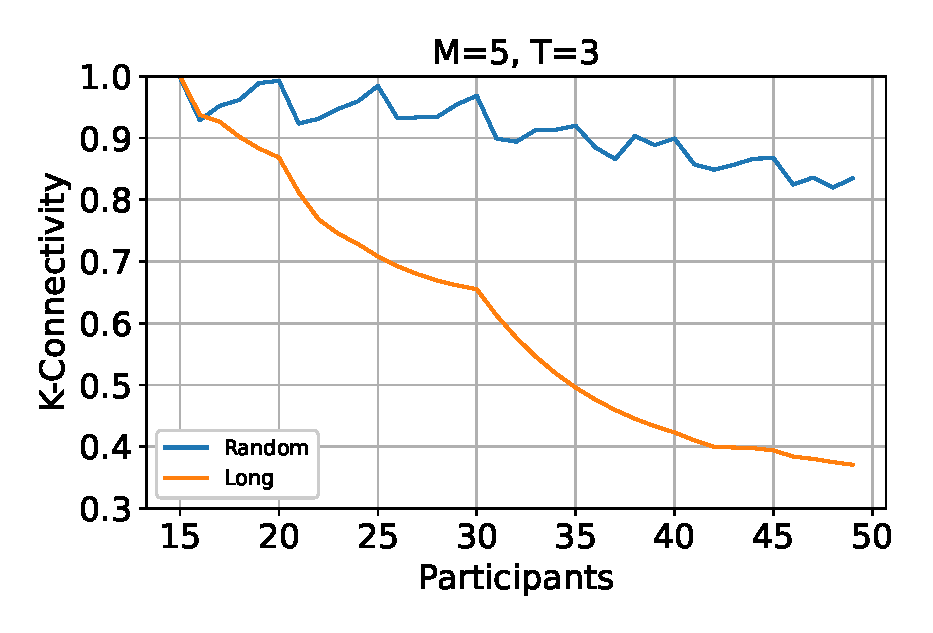
\includegraphics[width=5in]{fig/Experiment/fig-kcon.eps}
\caption{The k-connectivity of long-path and random-pod network deliberation
networks for $T=3$ stages and a pod size of $M=5$.}
\end{figure}

\subsection{Quantifying Preferences, Conflict, and Agreement}

\section{Study Software}

\section{Pilot Studies}
Several pilot studies have already been conducted:
one in a synchronous lab setting, and two using the asynchronous online
software.
In addition to providing an opportunity to test software,
these pilot studies have provided crucial information for developing a
feasible experimental design.

The initial pilot study was conducted on December 21, 2018,
before the custom online platform was developed.
In this pilot, NUMBER participants engaged in a synchronous 60-minute deliberation.
Participants sat at individual computer workstations, separated by dividers.
Participants discussed the following question:
``Where should the use of electric scooters be permitted?''
Participants were placed in a single treatment group, and divided into 4
pods of size 4--5.
These pods were reassigned using the random-pod method for a total of three
rounds.
The deliberation took place in chat rooms running the free and open-source
OTree online experiment software.

The second pilot took place after the initial development of the custom online
platform, from August 24, 2020 through August 32, 2020.

The third pilot took place from August 23, 2021 through August 29, 2021.



\chapter{Discussion}
\label{chap:discussion}
The assumption that coordination requires coercive hierarchy is so pervasive
that it is common to see the words ``hierarchy'' and ``organization'' used
interchangeably, as in the conventional ``org chart.''
Hierarchy is certainly a well-demonstrated tool for achieving coordination,
but that coordination comes with costs.
In terms of principles, hierarchical organizations rely on coercion and power imbalances,
sacrificing egalitarianism.
More practically, when information is distributed but decision-making is centralized,
that decision-making necessarily excludes potentially useful information.
The emergence of successful large-scale, internet-enabled, non-hierarchical collaborations
suggests that perhaps, at leaast in some cases,
neither the principle of egalitarianism nor the practical wisdom of the
crowd needs to be sacrificed to achieve effective coordination and collaboration.
The key question is: how do such large-scale participatory projects achieve success?

The work described and proposed here is motivated by and founded on empirical observations,
but it is also speculative in nature.
By employing agent-based models and experiment, it is possible to understand
not just how things are, but how things could be.
Rather than seeking to identify principles that apply broadly to existing
collaborations, this work starts from empirical observations of collaborations
that have done something unusual and attempts to identify robust principles
that might be applied to transform existing collaborations or create new ones.
The repeated appearance of small interlocking groups in successful large-scale
participatory collaborations suggests that this type of network structure might
be such a principle.
It may seem counterintuitive or even impossible that collaborations and organizations might deliberately
alter their interpersonal network structure.
But in fact, countless practices such as job interviews, letters of recommendation,
performance reviews, internships, mentorships, etc. all serve exactly this purpose;
to deliberately shape the social network within a collaboration.
By analogy, the task of deliberately designing a neighborhood might seem impossible,
but urban planners have made a science of it.

Between the completed chapters of this dissertation, a few commonalities emerge.
While it is conventional to describe the ``quality'' of a collaborive output,
both Chapter \ref{chap:wp-prod-perf} and Chapter{chap:abm} demonstrate that
quality can be multidimensional.
Specifically, Chapter \ref{chap:wp-prod-perf} shows that productivity and performance can
be anti-correlated in some contexts and not in others.
Similarly, Chapter \ref{chap:abm} identifies contexts where altering network structure
and social learning strategies can improve just performance, just productivity, or both.
Another common theme is that subtle differences in task or behavior can have dramatic
influences on output quality.
With regards to network deliberation in particular, Chapter \ref{chap:abm} suggests
that it is most effective in collaborations with a tendancy towards conformity.
Such conformity might occur because of social norms, or to compensate for sparse information.
Interestingly, the correlations between network properties and performance on Wikipedia
were consistent with a conformity-based social learning strategy.
Why network deliberation seems to improve conformity-based collaboration remains an
open question for future work.
And whether network deliberation has a similar effect in a controlled experimental
setting is yet to be seen.

While this work only scratches the surface of factors contributing to successful collaboration,
especially in the messiness of the real world, it identifies previously overlooked distinctions
that may help refine the study of participatory collaboration. Furthermore, starting from empirical
observation of large-scale participatory collaborations, this work has identified, refined, and formalized
network deliberation, and shown that, at least in agent based models, exhibits a distinct influence
on collaborative outcomes, independent of other network properties.
The ongoing work described in Chatper \ref{chap:experiment} will shed light on whether network deliberation
plays a causal role in enabling large-scale participatory collaborations.



%\chapter*{Acknowledgements}
%\include{acknoledgements.tex}


\begin{appendices}

\chapter{The NK-Model}
\label{apx:nk}
The NK Model \cite{kauffman_towards_1987} is an optimization problem particularly well-suited for modelling complex tasks. The model is used to create a fitness function $Q(s)$ over some discrete space $\mathcal{S}$, typically binary strings of a fixed length.
The model is parameterized by two variables.
The first, $N$, is the dimension of the solution space, i.e., the length of each binary string.
The second parameter, $K$, determines the ``ruggedness'' of the fitness function, i.e., the number of local maxima.
In effect, the $K$ parameter allows the complexity of the optimization problem to be tuned.
The ability to tune task complexity makes the NK model well-suited for studying the role of complexity in various settings.
The construction of an NK fitness function from a set of parameters is a stochastic process.
So particular values of $N$ and $K$ define a class of fitness functions, which can be sampled to produce a specific fitness function.

We now show the construction of the NK model fitness function.
A class of NK model fitness functions can be defined by a tuple of integer parameters
$(N, K)$ such that $N > 0$ and $0 \leq K < N$.
We begin by defining $N$ fitness contributions functions:
\begin{eqnarray}
q_i &:& \mathbb{Z}^{K+1} \rightarrow [0, 1].
\end{eqnarray}
The value of each $q_i(x)$ is chosen uniformly at random in the range $[0, 1]$ at the time the function is defined.
We also define $N$ projection operators $P_i$ which select $K+1$ bits from a length-$N$ bit string.
Each $P_i$ selects the bit at index $i$ and $K$ other indices, chosen uniformly at random at the time $P_i$ is constructed.
For a solution $s$, the $i$th fitness contribution is evaluated on the $K + 1$ bits selected by the $i$th projection: $q_i(P_i(s))$.
The value of the fitness function is the mean of all fitness contributions:
\begin{eqnarray}
Q(s) &=& \frac{1}{N}\sum_{i=1}^N q_i(P_i(s)).
\end{eqnarray}

The parameter $K$ alters the ruggedness of the fitness function by controlling the interdependence between the $q_i$.
When $K = 0$, each $q_i$ depends on a single unique index of $s$,
allowing the $q_i$ to be optimized independently.
In this case, $Q(s)$ has a single maximum: the global maximum.
However, for $K > 0$, two things happen: it becomes possible for each $q_i$ to have multiple local maxima, and some of the $q_i$ become coupled due to dependence on the same indices of $s$.
The result is that as $K$ increases, both the number of local maxima of $Q(s)$ \cite{weinberger_local_1991} and the difficulty of simultaneously optimizing the $q_i$ increase.
In other words, $Q$ becomes more rugged, and more complex.

The distribution of local maximum values is asymptotically normal for large $K$ \cite{weinberger_local_1991}.
When a skewed distribution is preferred, it is common to exponentiate the value of $Q(s)$ as a final step \cite{lazer_network_2007, barkoczi_social_2016, gomez_clustering_2019}.



\chapter{Interview Script}
\label{apx:interview}
\section{Preamble}

Hi! Thank you so much for taking time out to talk to us today. We appreciate it. Today we are here to understand how you use the internet to discuss complex issues and your experience participating in our discussion study.

\section{Warm-Up}

\begin{enumerate}
\item How often do you discuss political and policy issues with others, in general?
\item Where and how do you discuss those political and policy issues?
\item Which online social networks, forums, email lists, etc. do you regularly participate in?
\item In general, what have your experiences discussing politics and policy online been like?
\item Do you have any memorable experiences discussing an issue online?
\end{enumerate}

\section{Main Questions}

\begin{enumerate}
\item Reminder of topic, number of stages, length of stages
\item Going into the deliberation, what was your goal?
\item Overall, how would you describe your experience?
\item Do any memorable moments stand out to you?
\item How did it compare to other group deliberations you have participated in? 
\item What was your opinion in at the beginning of the deliberation?
\item What types of opinions did you encounter from other participants?
\begin{enumerate}
\item (follow-up) Can you walk me through how your opinions evolved throughout the deliberation?
\end{enumerate}
\item How much consensus existed at the beginning of the deliberation?
\begin{enumerate}
\item (follow-up) Can you walk me through how the group consensus evolved throughout the deliberation? 
\end{enumerate}
\item Did you witness or experience disagreement throughout the study?
\begin{enumerate}
\item (follow-up) Can you describe how disagreements and conflicts were addressed during deliberation? 
\item (follow-up) What is your opinion of the way disagreements and conflicts were addressed? (If clarification needed: was the process pleasant or unpleasant? Was it effective?)
\end{enumerate}
\item Did you share all of your thoughts with your groups?
\begin{enumerate}
\item (If the participant answers no) What do you think were the reasons?
\end{enumerate}
\item How often did you read posts by other participants? 
\item How often did you read replies to posts by other participants?
\item How often did you reply to posts by other participants?
\item What was your experience like when replying to previous comments?
\end{enumerate}

\section{Debrief}

\section{Final Questions}

\begin{enumerate}
\item Do you have any feedback on how to improve the system?
\end{enumerate}

\end{appendices}

\nocite{*}
\bibliographystyle{apacite}
\bibliography{proposal}

\end{document}
